% ============================================================
% Rozdział 3 — Implementacja i oryginalne rozwiązania techniczne
% Plan: docs/chapter3_plan.md
% ============================================================

Przejście od matematycznego opisu dynamiki cieczy do działającej implementacji
obliczeniowej jest samo w sobie wyzwaniem inżynierskim. Równania różniczkowe
opisujące zachowanie cieczy są precyzyjne i eleganckie; ich dyskretyzacja oraz
wykonanie na rzeczywistym sprzęcie odsłaniają natomiast ograniczenia, które
w modelu teoretycznym nie istnieją. Każdy krok symulacji musi zostać
zdekomponowany na operacje równoległe wykonywane przez tysiące wątków GPU,
a ta równoległość niesie ze sobą nowe klasy problemów nieobecne w algorytmach
sekwencyjnych: równoczesny odczyt i zapis buforów, konieczność koherencji
pamięci podręcznej, wrażliwość na wzorzec dostępu do pamięci globalnej.

Implementacja w modelu GPGPU (ang.~\textit{General-Purpose computing on Graphics Processing Units}) 
nie jest przepisaniem algorytmu sekwencyjnego
na kod shaderów. Wymaga świadomego projektowania struktur danych pod kątem
przepustowości pamięci, doboru algorytmów sortowania dostosowanych do
architektury SIMT (ang.~\textit{Single Instruction, Multiple Threads}), 
zarządzania synchronizacją między etapami potoku
obliczeniowego oraz kontroli arytmetyki zmiennoprzecinkowej, której błędy
akumulacji mogą zdestabilizować pozornie poprawną symulację.

Niniejszy rozdział przedstawia implementację silnika symulacji cieczy opartego
na metodzie DFSPH, realizowanej na GPU, w formie ciągu wyzwań i kompromisów
technicznych. Każda decyzja projektowa --- od wyboru struktury danych
i algorytmu sortowania, przez strategię doboru kroku czasowego, po architekturę
potoku renderowania --- jest uzasadniona analizą strukturalną lub bezpośrednim
pomiarem.

% ------------------------------------------------------------
\section{Założenia projektowe}
\label{sec:assumptions}

Uruchomienie silnika wymaga spełnienia wymagań sprzętowych i programowych
opisanych poniżej. Projekt jest przeznaczony wyłącznie dla systemu Windows ---
kod źródłowy korzysta z rozszerzenia \texttt{winit::platform::windows}, które
udostępnia funkcjonalności specyficzne dla tej platformy
(m.in.\ ikona na pasku zadań), co wyklucza kompilację na systemach Linux
i macOS bez uprzedniej modyfikacji.

Wymagania sprzętowe i programowe zestawiono odpowiednio
w tabelach~\ref{tab:hw_requirements} i~\ref{tab:build_requirements}.

\begin{table}[H]
\centering
\caption{Wymagania sprzętowe}
\label{tab:hw_requirements}
\begin{tabular}{lp{8cm}}
\toprule
\textbf{Komponent} & \textbf{Wymaganie} \\
\midrule
GPU & Obsługa Vulkan 1.3 (karty graficzne klasy GTX~1000 / RX~400 lub nowsze) \\[4pt]
System operacyjny & Windows 10 w wersji 2004 lub nowszy \\[4pt]
Sterownik GPU & Aktualny sterownik producenta z obsługą Vulkan 1.3 \\
\bottomrule
\end{tabular}
\end{table}

\begin{table}[H]
\centering
\caption{Wymagania do kompilacji}
\label{tab:build_requirements}
\begin{tabular}{ll}
\toprule
\textbf{Narzędzie} & \textbf{Wersja minimalna} \\
\midrule
Rust (edycja 2024) & 1.85 \\
Kompilator C++ & MSVC (Visual Studio Build Tools) \\
Vulkan SDK & 1.3.x (zawiera \texttt{shaderc}) \\
\bottomrule
\end{tabular}
\end{table}

Kompilator C++ jest wymagany przez bibliotekę \texttt{tracy-client}
z włączoną funkcją \texttt{enable}, która kompiluje bibliotekę profilowania
Tracy ze źródeł C++. Shadery GLSL są kompilowane do formatu SPIR-V
w czasie budowania projektu przez bibliotekę \texttt{vulkano-shaders},
korzystającą z narzędzia \texttt{shaderc} dołączonego do Vulkan SDK.

Silnik oczekuje obecności następujących plików w katalogu projektu:
\begin{itemize}
    \item \texttt{assets/logo.png} --- ikona okna i paska zadań,
    \item \texttt{assets/hdri/citrus\_orchard\_road\_puresky\_4k.exr} ---
          panorama HDRI w formacie OpenEXR, używana jako środowisko
          oświetleniowe i tło sceny.
\end{itemize}

% ------------------------------------------------------------
\section{Architektura systemu}
\label{sec:architecture}

Silnik jest podzielony na dwie warstwy: warstwę CPU, która orkiestruje
wykonanie i zarządza stanem aplikacji, oraz warstwę GPU, która realizuje
wszystkie obliczenia fizyczne i renderowanie. Procesor nie wykonuje żadnych
obliczeń symulacji --- jego jedyną rolą jest zbudowanie buforów komend
Vulkan i przesłanie ich do kolejki GPU. Podział modułów między obie warstwy
przedstawia tabela~\ref{tab:subsystems}.

\begin{table}[H]
\centering
\caption{Podział modułów systemu}
\label{tab:subsystems}
\begin{tabular}{lp{2.5cm}p{7cm}}
\toprule
\textbf{Moduł} & \textbf{Platforma} & \textbf{Rola} \\
\midrule
\texttt{Engine}            & CPU          & Pętla zdarzeń winit, timing, zarządzanie sceną i wejściem \\[3pt]
\texttt{Scene}             & CPU          & Parametry symulacji, pozycje startowe cząstek, kamera, granice kolizji \\[3pt]
\texttt{Controller}        & CPU          & Odwzorowanie klawiatury i myszy na obiekty komend \\[3pt]
\texttt{Renderer}          & CPU          & Budowanie buforów komend Vulkan, synchronizacja faz fizyki i renderowania \\[3pt]
\texttt{GpuSceneResources} & GPU          & Bufory cząstek, parametry symulacji, tekstury, dane kamery \\[3pt]
\texttt{ComputePipelines}  & GPU          & 11 potoków obliczeniowych realizujących solver DFSPH \\[3pt]
\texttt{Pipelines}         & GPU          & Potoki graficzne: niebo, cząsteczki, woda (ray marching), granice \\
\bottomrule
\end{tabular}
\end{table}

Pętla ramki jest sterowana zdarzeniem \texttt{RedrawRequested} biblioteki
winit i wykonuje się w trybie \texttt{ControlFlow::Poll}, co oznacza brak
ograniczenia liczby klatek przez system operacyjny. Algorytm~\ref{alg:frame_loop}
przedstawia kolejność operacji w obrębie jednej klatki.

\begin{algorithm}[H]
\caption{Pętla ramki}
\label{alg:frame_loop}
$\Delta t \leftarrow \texttt{fps\_counter.tick()}$\;
$\Delta t_{\text{bezp}} \leftarrow \min(\Delta t,\ 0{,}1\,\text{s})$\;
\If{\upshape okno sfokusowane}{
    wykonanie komend z \texttt{Controller} na obiektach \texttt{Scene}\;
}
\tcp{Faza fizyki --- GPU}
odczytanie statystyk z poprzedniej klatki ($v_{\max}$, błąd gęstości, błąd dywergencji)\;
\If{\upshape tryb CFL\footnotemark{} włączony \upshape \textnormal{i} $v_{\max} > 0{,}01$}{
    $dt \leftarrow \mathrm{clamp}(0{,}4 \cdot h / v_{\max},\ 0{,}001,\ 0{,}05)$\;
    $dt \leftarrow \min(dt,\ dt_{\text{poprzedni}} \cdot 1{,}1)$\;
}
uruchomienie \texttt{neighbor\_search}, \texttt{density\_alpha}\;
$t \leftarrow 0$\;
\While{$t < \Delta t_{\text{bezp}}$}{
    uruchomienie \texttt{viscosity}, \texttt{density\_source\_term}\;
    \For{$i \leftarrow 1$ \KwTo $N_{\rho}$}{
        uruchomienie \texttt{pressure\_force}, \texttt{pressure\_update}\;
    }
    uruchomienie \texttt{pressure\_integration}\;
    $t \leftarrow t + dt$\;
    uruchomienie \texttt{neighbor\_search}, \texttt{density\_alpha}\;
    uruchomienie \texttt{divergence\_source\_term}\;
    \For{$i \leftarrow 1$ \KwTo $N_{\nabla\!v}$}{
        uruchomienie \texttt{pressure\_force}, \texttt{pressure\_update}\;
    }
    uruchomienie \texttt{divergence\_integration}\;
}
uruchomienie \texttt{stats}\;
skopiowanie pozycji i kolorów cząstek do bufora renderowania\;
\tcp{Faza renderowania --- GPU}
\If{\upshape tryb ray marching}{
    uruchomienie \texttt{density\_texture}\;
}
narysowanie nieba, wody (lub cząstek), granic kolizji\;
nałożenie interfejsu użytkownika (egui)\;
zaprezentowanie klatki\;
\end{algorithm}
\footnotetext{CFL --- warunek Couranta–Friedrichsa–Lewy'ego
(ang.~\textit{Courant--Friedrichs--Lewy condition})~\cite{lax2013stability};
szczegóły w podrozdz.~\ref{subsec:cfl}}

W implementacji zastosowano cztery wzorce projektowe.
\textit{ApplicationHandler} odwraca kontrolę nad pętlą zdarzeń --- zamiast
silnik samodzielnie odpytywał kolejkę komunikatów, to system operacyjny
wywołuje jego metody w odpowiedzi na zdarzenia okna i urządzeń wejściowych.
\textit{ComputeStep} nadaje wszystkim potokom obliczeniowym GPU jednolity
interfejs, rozdzielając jednorazową inicjalizację zasobów od wielokrotnie
powtarzanego zapisu poleceń do bufora komend.
\textit{Command} oddziela detekcję wejścia od modyfikacji stanu --- każde
naciśnięcie klawisza lub ruch myszy przekładane są na obiekt komendy, który
wie, jak zmienić scenę, ale nie wie, skąd pochodzi sygnał.
\textit{Actor} abstrahuje przemieszczanie i obrót w przestrzeni 3D
w sposób niezależny od konkretnego obiektu sceny.

% ------------------------------------------------------------
\section{Warstwa aplikacji}
\label{sec:app_layer}

Zanim GPU wykona choćby jeden krok symulacji, warstwa CPU musi otworzyć
okno, przetworzyć wejście użytkownika i zsynchronizować parametry sceny
z pamięcią karty graficznej. Trzy moduły odpowiadają za te zadania:
biblioteka winit zarządzająca oknem i pętlą zdarzeń, model kamery
przekształcający ruch myszy w macierze widoku, oraz struktura sceny,
która stanowi jedyne źródło parametrów przekazywanych do każdego shadera.

\subsection{Zarządzanie oknem}
\label{subsec:window}

Okno i pętla zdarzeń są obsługiwane przez bibliotekę winit za pośrednictwem
cechy \textit{ApplicationHandler}. Zamiast samodzielnej pętli \texttt{while},
silnik implementuje tę cechę i przekazuje sterowanie systemowi zdarzeń ---
jest to wzorzec odwrócenia kontroli, w którym to system operacyjny wywołuje
metody aplikacji w odpowiedzi na zdarzenia.

Metoda \texttt{resumed()} należy do modelu cyklu życia \textit{ApplicationHandler}
i jest wywoływana za każdym razem, gdy aplikacja przechodzi ze stanu
zawieszonego do aktywnego. Na platformach bez jawnego cyklu zawieszania,
takich jak Windows, zdarzenie to jest emitowane jednorazowo po inicjalizacji
i pełni rolę sygnału startu. Na platformach mobilnych może być wywoływana
wielokrotnie --- na Androidzie tworzenie powierzchni renderowania
przed tym zdarzeniem jest niemożliwe. Winit zaleca\cite{winit} więc inicjalizację okna
i kontekstu graficznego dopiero w odpowiedzi na pierwsze \texttt{Resumed},
co w kodzie przekłada się na tworzenie obiektów \texttt{Window}
i \texttt{Renderer} wewnątrz tej metody. Metoda \texttt{window\_event()} obsługuje wszystkie
zdarzenia okna, a metoda \texttt{device\_event()} przechwytuje ruch myszy
jako surowe przesunięcia, niezależnie od pozycji kursora.

Silnik rozróżnia dwa stany okna: \textit{aktywny} --- kursor widoczny,
brak obsługi wejścia z kamery --- oraz \textit{sfokusowany} --- kursor
ukryty i zablokowany, aktywna kamera. Przejście do trybu sfokusowanego
następuje przez kliknięcie lewym przyciskiem myszy lub zdarzenie
\texttt{Focused(true)}; powrót do trybu aktywnego --- przez naciśnięcie
klawisza Escape lub zdarzenie \texttt{Focused(false)}.

Pętla działa w trybie \texttt{ControlFlow::Poll}, co oznacza, że
\texttt{RedrawRequested} jest generowane natychmiast po każdej iteracji bez
oczekiwania na zdarzenia systemowe. Swapchan używa trybu \texttt{PresentMode::Immediate}, który wyświetla
ukończoną klatkę natychmiast, bez oczekiwania na sygnał synchronizacji
pionowej. Liczba obrazów swapchaina wynosi 3; stała
\texttt{MAX\_FRAMES\_IN\_FLIGHT = 3} ogranicza liczbę ramek budowanych
przez CPU równolegle z pracą GPU --- razem tworzą pełny triple buffering.

\subsection{Kamera}
\label{subsec:camera}

Kamera jest podzielona na dwie struktury. \texttt{Camera} przechowuje stan
logiczny po stronie CPU; \texttt{CameraGPU} zawiera dane gotowe
do przesłania na GPU. Pola obu struktur opisują
tabele~\ref{tab:camera_cpu} i~\ref{tab:camera_gpu}.

\begin{table}[tp]
\centering
\caption{Pola struktury \texttt{Camera}}
\label{tab:camera_cpu}
\begin{tabular}{llp{7cm}}
\toprule
\textbf{Pole} & \textbf{Typ} & \textbf{Opis} \\
\midrule
\texttt{position}     & \texttt{Vec3}  & Położenie obserwatora w przestrzeni świata \\[3pt]
\texttt{orientation}  & \texttt{Quat}  & Orientacja przestrzenna; kwaternion jest standardową reprezentacją obrotu w grafice 3D \\[3pt]
\texttt{fov}          & \texttt{f32}   & Kąt widzenia (ang. \textit{field of view}, 45°) --- kąt między lewą a prawą krawędzią pola widzenia; większy kąt daje szerszy widok, ale silniejsze zniekształcenie perspektywiczne na brzegach \\[3pt]
\texttt{aspect\_ratio}& \texttt{f32}   & Proporcje ekranu, domyślnie 16/9 \\[3pt]
\texttt{near} / \texttt{far} & \texttt{f32} & Bliższa i dalsza płaszczyzna obcinania (ang. \textit{clipping planes}, 0.1~m i 1000.0~m) --- przedział odległości, w którym GPU renderuje geometrię; obiekty spoza tego przedziału są pomijane \\
\bottomrule
\end{tabular}
\end{table}

\begin{table}[tp]
\centering
\caption{Pola struktury \texttt{CameraGPU} przesyłanej na GPU}
\label{tab:camera_gpu}
\begin{tabular}{llp{6.5cm}}
\toprule
\textbf{Pole} & \textbf{Typ} & \textbf{Opis} \\
\midrule
\texttt{view}           & \texttt{Mat4} & Macierz widoku --- przekształca punkty z przestrzeni świata do przestrzeni kamery \\[3pt]
\texttt{proj}           & \texttt{Mat4} & Macierz projekcji --- odwzorowuje przestrzeń kamery na NDC \\[3pt]
\texttt{inv\_view\_proj}& \texttt{Mat4} & Odwrotność $(\mathbf{P}\mathbf{V})^{-1}$ --- używana przez ray marching do odtworzenia kierunku promienia \\[3pt]
\texttt{camera\_pos}    & \texttt{Vec3} & Pozycja kamery w przestrzeni świata (+ 4~bajty wyrównania) \\
\bottomrule
\end{tabular}
\end{table}

Obrót kamery stosuje podejście charakterystyczne dla kamer pierwszoosobowych.
Obrót wokół osi Y {odchylenie} (ang.~\textit{yaw}) jest aplikowany
w przestrzeni globalnej, a wokół osi X pochylenie (ang.~\textit{pitch}) --- w przestrzeni lokalnej kamery:
\begin{equation}
  q_{\text{new}} = q_{\text{yaw}} \cdot q_{\text{current}} \cdot q_{\text{pitch}}
  \label{eq:camera_rot}
\end{equation}
Dzięki temu linia horyzontu pozostaje zawsze pozioma, a obrót nie kumuluje
skręcenia wzdłuż osi Z.

Bufor kamery jest tworzony z flagą \texttt{SHADER\_DEVICE\_ADDRESS}, co
pozwala przekazywać go do shaderów jako surowy adres GPU zamiast wiązać
przez deskryptor. Macierz widoku wyznaczana jest funkcją
\texttt{look\_at\_lh} na podstawie pozycji i orientacji kamery, macierz
projekcji --- funkcją \texttt{perspective\_lh},
a \texttt{inv\_view\_proj}\cite{glam} stanowi odwrotność ich iloczynu $(\mathbf{P}\mathbf{V})^{-1}$.
Rysunek~\ref{fig:camera_chain} ilustruje kolejność tych obliczeń.

\begin{figure}[h]
\centering
\begin{tikzpicture}[
  box/.style={draw, rounded corners=3pt, minimum width=5cm,
              minimum height=0.85cm, align=center, font=\small},
  >=Stealth, node distance=0.55cm
]
  \node[box] (state) {\texttt{position}, \texttt{orientation}};
  \node[box, below=of state] (view) {macierz widoku};
  \node[box, below=of view]  (proj) {macierz projekcji};
  \node[box, below=of proj]  (inv)  {\texttt{inv\_view\_proj}};
  \node[box, below=of inv]   (buf)  {\texttt{CameraGPU}};
  \draw[->] (state) -- (view);
  \draw[->] (view)  -- (proj);
  \draw[->] (proj)  -- (inv);
  \draw[->] (inv)   -- (buf);
\end{tikzpicture}
\caption{Łańcuch obliczeń kamery\newline Źródło: Opracowanie własne}
\label{fig:camera_chain}
\end{figure}

Macierz \texttt{inv\_view\_proj} jest potrzebna dla ray marchingu. Shader
operuje na współrzędnych NDC (ang. \textit{Normalized Device Coordinates}) ---
układzie, w którym środek ekranu to $(0,\,0)$, a narożniki $(\pm1,\,\pm1)$.
Aby wyznaczyć kierunek promienia dla danego piksela, shader mnoży jego
współrzędne NDC przez \texttt{inv\_view\_proj} i odejmuje pozycję kamery ---
bez żadnych dodatkowych przesyłań danych między CPU a GPU.

Vulkan definiuje układ NDC z osią Y skierowaną w dół\cite{vulkan-spec}, odwrotnie niż OpenGL,
co powoduje, że obraz renderowany standardową macierzą projekcji jest
odwrócony pionowo. Zamiast modyfikować macierze, problem rozwiązuje odwrócenie
okienka renderowania (ang. \textit{viewport}) --- prostokątnego obszaru okna,
na którym GPU wyświetla wynik. W implementacji ustawiono ujemną wysokość okienka przy przesuniętym
punkcie startowym, co przesuwa układ do konwencji Y-w-górę bez żadnych
zmian w shaderach ani macierzach.

\subsection{Scena i parametry symulacji}
\label{subsec:scene_params}

Struktura \texttt{Scene} grupuje cztery elementy: wektor startowych pozycji
cząstek, strukturę \texttt{SimulationParams}, obiekt kamery oraz granice
kolizji (\texttt{CollisionBox}). Jest jedynym źródłem danych konfiguracyjnych
--- wszystkie shadery odczytują parametry wyłącznie z bufora
\texttt{sim\_params\_buffer}, który jest odświeżany na początku każdej klatki
wywołaniem \texttt{sync\_with\_scene()}.

Tabela~\ref{tab:sim_params} zestawia parametry struktury \texttt{SimulationParams}
wraz z wartościami domyślnymi ustawionymi w konstruktorze \texttt{Scene::new()}.

\begin{table}[H]
\centering
\caption{Parametry symulacji i ich wartości domyślne}
\label{tab:sim_params}
\begin{tabular}{p{4.0cm}ll}
\toprule
\textbf{Parametr} & \textbf{Wartość domyślna} & \textbf{Opis} \\
\midrule
\texttt{particle\_radius}   & 0.020~m       & Promień cząstki \\
\texttt{smoothing\_radius}  & 0.080~m       & Zasięg jądra SPH ($= 4r$) \\
\texttt{target\_density}    & 1000~kg/m³    & Gęstość referencyjna \\
\texttt{dt}                 & 0.005~s       & Stały krok czasowy \\
\texttt{viscosity}          & 0.15          & Współczynnik XSPH \\
\texttt{relax\_factor}      & 0.5           & Współczynnik relaksacji solvera \\
\texttt{density\_solver\_}\newline\texttt{iterations}    & 4 & Iteracje korekcji gęstości \\
\texttt{divergence\_solver\_}\newline\texttt{iterations} & 4 & Iteracje korekcji dywergencji \\
\texttt{gravity}            & $(0,\,-9{,}81,\,0)$~m/s² & Przyspieszenie grawitacyjne \\
\texttt{grid\_res}          & $128^3$       & Rozdzielczość siatki przestrzennej \\
\bottomrule
\end{tabular}
\end{table}

% ------------------------------------------------------------
\section{Inicjalizacja GPU z Vulkano}
\label{sec:gpu_init}

Konfiguracja Vulkan silnika skupia się wokół dwóch elementów:
doboru minimalnego zestawu funkcji urządzenia wymaganych przez solver
DFSPH oraz autorskiej cechy \texttt{ComputeStep} --- oryginalnej warstwy
abstrakcji, która nadaje wszystkim potokom obliczeniowym jednolity
cykl życia: jednorazową kompilację shadera przy starcie i ustandaryzowany
zapis poleceń do bufora komend co klatkę.

\subsection{Kontekst Vulkan}
\label{subsec:vulkan_context}

W podrozdziale~\ref{sec:vulkan_hierarchy} opisano hierarchię inicjalizacyjną
Vulkan --- instancja, urządzenie fizyczne, urządzenie logiczne, kolejki
--- jako sekwencję jawnych operacji. W kodzie ta hierarchia jest ukryta
za strukturą \texttt{VulkanoConfig}: silnik wypełnia ją listą potrzebnych
funkcji i rozszerzeń, a \texttt{VulkanoContext::new()} przeprowadza całą
inicjalizację, wybierając urządzenie i budując obiekty niskopoziomowe.

Wymagania solvera narzuciły trzy funkcje obliczeniowe.
\texttt{buffer\_device\_address} pozwala shaderom pobierać dane
bezpośrednio ze wskazanego adresu w pamięci GPU zamiast przez deskryptor
--- bufor kamery jest przekazywany jako wskaźnik bezpośredni, co eliminuje
konieczność deklarowania zestawu deskryptorów dla jednego bufora. Rozszerzenie
\texttt{scalar\_block\_layout} wymusza wyrównanie pól struktur GLSL
zgodne z~układem C --- bez tej funkcji kompilator GLSL może wstawiać
wypełnienie (ang.~\textit{padding}) między polami inaczej niż Rust,
co powoduje odczyt błędnych wartości z buforów fizyki.
\texttt{shader\_int64} jest potrzebny do operacji indeksowania
w shaderach obliczeniowych.

Warstwa renderowania wprowadziła dodatkowe wymagania techniczne. Funkcja
\texttt{dynamic\_rendering} --- opisana w podrozdziale~\ref{sec:vulkan_swapchain}
jako alternatywa dla jawnych obiektów RenderPass --- eliminuje konieczność
deklarowania kompatybilności potoków z konkretnym formatem framebuffera.
\texttt{large\_points} i \texttt{fill\_mode\_non\_solid} pozwalają
przełączać tryb wizualizacji cząstek --- renderowanie jako punkt, bryłę
lub siatkę --- bez przebudowy potoków.
Filtrowanie anizotropowe (ang.~\textit{anisotropic filtering}),
aktywowane przez \texttt{sampler\_anisotropy}, kompensuje rozmycie
tekstur oglądanych pod ukośnym kątem --- bez niego panorama HDRI
traci szczegółowość w obszarach, gdzie promień kamery pada pod małym
kątem do powierzchni.
Rozszerzenie instancji \texttt{ext\_debug\_utils} aktywuje warstwy
walidacyjne opisane w sekcji~\ref{sec:dev_tools} --- w trakcie tworzenia
silnika wielokrotnie ujawniały one błędy synchronizacji niewidoczne
w standardowym wyjściu.

Obsługę łańcucha wymiany i powierzchni renderowania powierzono komponentowi
\texttt{VulkanoWindowRenderer}\cite{vulkano-rs}. Definiuje on ścisły cykl
życia klatki oparty na parze operacji \texttt{acquire} i \texttt{present}.
Metoda \texttt{acquire} pobiera indeks dostępnego obrazu ze swapchainu
i zwraca obiekt synchronizacji; po zarejestrowaniu i przesłaniu wszystkich
buforów poleceń wywołanie \texttt{present} kolejkuje obraz do wyświetlenia,
przekazując gotowy wynik do menedżera okien systemu operacyjnego.

\subsection{Wzorzec ComputeStep}
\label{subsec:compute_step}

Gdy kontekst Vulkan jest skonfigurowany, silnik dysponuje urządzeniem
i kolejkami potrzebnymi do tworzenia potoków obliczeniowych. Każdy
potok wymaga tej samej sekwencji inicjalizacyjnej: załadowania shadera
SPIR-V, wyprowadzenia układu deskryptorów z jego refleksji i kompilacji
obiektu \texttt{ComputePipeline}. Cecha \texttt{ComputeStep} hermetyzuje
tę sekwencję w domyślnej implementacji \texttt{new()}; implementator
musi dostarczyć jedynie dwie metody --- ładującą skompilowany shader
oraz opakowującą gotowy obiekt potoku.
Listing~\ref{lst:compute_step} przedstawia pełną definicję cechy.

\begin{lstlisting}[caption={Cecha \texttt{ComputeStep}},
                   label=lst:compute_step]
pub trait ComputeStep: Sized {
    fn load_shader_module(device: Arc<Device>) -> EntryPoint;
    fn from_pipeline(pipeline: Arc<ComputePipeline>) -> Self;
    fn new(device: Arc<Device>) -> Self {
        let entry_point = Self::load_shader_module(device.clone());
        let stage = PipelineShaderStageCreateInfo::new(entry_point);
        let layout = PipelineLayout::new(
            device.clone(),
            PipelineDescriptorSetLayoutCreateInfo::from_stages(
                [&stage])
                .into_pipeline_layout_create_info(device.clone())
                .unwrap(),
        ).unwrap();
        let pipeline = ComputePipeline::new(
            device.clone(), None,
            ComputePipelineCreateInfo::stage_layout(stage, layout),
        ).unwrap();
        Self::from_pipeline(pipeline)
    }
    fn prepare(&mut self,
               allocator: Arc<StandardDescriptorSetAllocator>,
               physics_data: &GpuPhysicsData,
               sim_params: &Subbuffer<SimulationParams>);
    fn execute<Cb>(&self, 
                   builder: &mut AutoCommandBufferBuilder<Cb>);
}
\end{lstlisting}

Inicjalizacja potoku przebiega w trzech krokach.
Najpierw bajtkod SPIR-V shadera --- skompilowany już w czasie budowania
projektu przez \texttt{vulkano-shaders} --- jest ładowany do pamięci
i przekazywany jako punkt wejścia identyfikujący funkcję główną shadera.
Następnie \texttt{PipelineDescriptorSetLayoutCreateInfo::from\_stages}
analizuje ten bajtkod i automatycznie wyprowadza układ deskryptorów ---
tabelę opisującą GPU, ile buforów i tekstur potok odczytuje oraz pod
jakimi numerami wiązań je znajdzie; bez tej refleksji programista
musiałby deklarować tę tabelę ręcznie, duplikując informacje już zawarte
w shaderze.
Na końcu Vulkan kompiluje shader do natywnych instrukcji karty graficznej
i tworzy obiekt \texttt{ComputePipeline}, który pozostaje gotowy przez
cały czas życia aplikacji --- ta kompilacja zdarza się tylko raz, przy
starcie.

Metoda \texttt{prepare()} jest wywoływana jednorazowo przy starcie ---
przydziela zestaw deskryptorów i trwale wiąże z nim bufory fizyki;
deskryptory pozostają ważne przez cały czas życia aplikacji, bo bufory
nie są realokowane.
Co klatkę wywoływane jest wyłącznie \texttt{execute()}, które zapisuje
do buildera komend pojedyncze polecenie dispatchu --- żądanie uruchomienia
na GPU określonej liczby grup wątków obliczeniowych --- bez żadnych
alokacji ani zmiany stanu deskryptorów.

Razem implementatory cechy \texttt{ComputeStep} tworzą kompletny potok
obliczeniowy odpowiadający kolejnym etapom pętli ramki z
algorytmu~\ref{alg:frame_loop}.
Tabela~\ref{tab:compute_steps} zestawia wszystkich implementatorów
wraz z ich rolami.

\begin{table}[htbp]
\centering
\caption{Implementatory cechy \texttt{ComputeStep}}
\label{tab:compute_steps}
\begin{tabular}{p{6.5cm}p{7cm}}
\toprule
\textbf{Implementator} & \textbf{Rola} \\
\midrule
\texttt{GpuSorter}                     & Sortowanie cząstek po kluczu siatki przestrzennej \\[3pt]
\texttt{NeighborSearch}                & Budowanie siatki przestrzennej; deleguje sortowanie do \texttt{GpuSorter} \\[3pt]
\texttt{DensityAlphaPipeline}          & Gęstość SPH i współczynnik $\alpha$ \\[3pt]
\texttt{ViscosityPipeline}             & Lepkość XSPH i grawitacja \\[3pt]
\texttt{DensitySourceTermPipeline}     & Człon źródłowy korekcji gęstości \\[3pt]
\texttt{PressureForcePipeline}         & Siły ciśnienia w iteracji solvera \\[3pt]
\texttt{PressureUpdatePipeline}        & Aktualizacja pola ciśnienia \\[3pt]
\texttt{PressureIntegrationPipeline}   & Całkowanie prędkości po korekcji gęstości \\[3pt]
\texttt{DivergenceSourceTermPipeline}  & Człon źródłowy korekcji dywergencji \\[3pt]
\texttt{DivergenceIntegrationPipeline} & Całkowanie prędkości po korekcji dywergencji \\[3pt]
\texttt{StatsPipeline}                 & Statystyki klatki: $v_{\max}$, błędy gęstości i dywergencji \\[3pt]
\texttt{DensityTexturePipeline}        & Zapis gęstości do tekstury 3D  \\
\bottomrule
\end{tabular}
\end{table}

\subsection{Deskryptory i synchronizacja}
\label{subsec:descriptors}

Deskryptor (ang.~\textit{descriptor}) jest uchwytem wiążącym bufor lub
teksturę z punktem wiązania (ang.~\textit{binding}) zadeklarowanym
w shaderze. Aby GPU wiedziało, z jakiej pamięci pobrać dane podczas
wykonania shadera, każde polecenie dispatchu musi być poprzedzone
dowiązaniem zestawu deskryptorów.

Układ zestawu deskryptorów każdego potoku wyprowadzany jest automatycznie
przez vulkano z refleksji skompilowanego shadera SPIR-V --- bez ręcznej
deklaracji typów ani rozmiarów wiązań w kodzie Rust. Metoda
\texttt{prepare()} alokuje zestaw deskryptorów ze wspólnego
\texttt{StandardDescriptorSetAllocator} i wiąże z nim bufory fizyki
pobrane z \texttt{GpuPhysicsData}; ponieważ alokacja następuje wyłącznie
w \texttt{prepare()}, metoda \texttt{execute()} nie wykonuje żadnych
operacji na stercie.

Między kolejnymi dispatchami niezbędne są bariery pamięci
(ang.~\textit{pipeline barriers}), wymuszające widoczność zapisów
wykonanych przez poprzedni potok przed odczytem przez następny.
\texttt{AutoCommandBufferBuilder} wpisuje te bariery bezpośrednio
do bufora komend po każdym poleceniu dispatchu, gwarantując spójność
danych w całym potoku obliczeniowym.

% ------------------------------------------------------------
\section{Struktury danych cząstek}
\label{sec:data_structures}

Zanim możliwe jest zbudowanie potoku obliczeniowego, konieczne jest podjęcie
decyzji dotyczącej organizacji danych cząstek w pamięci GPU.
Wybór ten determinuje zarówno poprawność symulacji --- ze względu na model
pamięci Vulkan --- jak i wydajność obliczeniową, poprzez wpływ na wzorzec
dostępu do pamięci podręcznej procesorów strumieniowych.

\subsection{Organizacja danych: AOS i SOA}
\label{subsec:soa_aos}

Organizacja danych cząstek w pamięci GPU decyduje o wydajności każdego
kroku obliczeniowego --- shaderowy solver SPH odczytuje atrybuty
kilkudziesięciu sąsiadów dla każdej z tysięcy cząstek w każdej klatce.
Istnieją dwa fundamentalne układy: AOS (ang.~\textit{Array of Structures}),
w którym wszystkie atrybuty jednej cząstki leżą obok siebie, oraz SOA
(ang.~\textit{Structure of Arrays}), gdzie każdy atrybut tworzy osobny
bufor.

Listing~\ref{lst:aos} przedstawia hipotetyczny układ AOS zastosowany
w pierwszej wersji silnika, a listing~\ref{lst:soa} pokazuje faktyczny
układ SOA, do którego przejście okazało się konieczne.

\begin{lstlisting}[caption={Hipotetyczny układ AOS (porzucony)},
                   label=lst:aos]
struct Particle {
    position: [f32; 4],  // 16 B
    velocity: [f32; 4],  // 16 B
    density:  f32,       //  4 B
    factor:   f32,       //  4 B
    pressure: f32,       //  4 B
}
// bufor: [Particle; N] -- atrybuty przeplatane co 44 B
\end{lstlisting}

\begin{lstlisting}[caption={Kompletna struktura \texttt{GpuPhysicsData} -- układ SOA},
                   label=lst:soa]
pub struct GpuPhysicsData {
    pub count: u32,

    // podwojne buforowanie pozycji i predkosci
    pub position_a: Subbuffer<[[f32; 4]]>,
    pub position_b: Subbuffer<[[f32; 4]]>,
    pub velocity_a: Subbuffer<[[f32; 4]]>,
    pub velocity_b: Subbuffer<[[f32; 4]]>,

    pub colors:     Subbuffer<[[f32; 4]]>,

    // pola fizyczne solvera DFSPH
    pub densities:               Subbuffer<[f32]>,
    pub factors:                 Subbuffer<[f32]>,
    pub source_terms:            Subbuffer<[f32]>,
    pub pressures:               Subbuffer<[f32]>,
    pub pressure_accelerations:  Subbuffer<[[f32; 4]]>,

    // siatka przestrzenna (wyszukiwanie sasiadow)
    pub grid_entries: Subbuffer<[Entry]>,
    pub grid_start:   Subbuffer<[u32]>,

    // v_max, blad gestosci, blad dywergencji
    pub stats_buffer: Subbuffer<[u32]>, 
}
\end{lstlisting}

Bezpośrednią przyczyną porzucenia układu AOS był błąd ujawniający się
natychmiast po uruchomieniu pierwszej wersji solvera.
Shader obliczający nowe prędkości cząstek odczytywał prędkości sąsiednich
cząstek i jednocześnie zapisywał zaktualizowane wartości do tego samego
bufora.
Vulkan traktuje taki wzorzec odczytu-zapisu bez odpowiedniej bariery
jako nieokreślone zachowanie --- wynik zależy od wewnętrznej kolejności
wykonania wątków GPU, która nie jest gwarantowana.
W praktyce część wątków odczytywała już zaktualizowane wartości sąsiadów
zamiast wartości sprzed kroku, co prowadziło do niestabilnych wyników
lub zgłoszenia błędu walidacji przez bibliotekę Vulkano.

Układ SOA rozwiązuje ten problem strukturalnie: każdy atrybut fizyczny
zajmuje osobny bufor, a pozycje i prędkości wyposażono w dodatkowe bufory
umożliwiające technikę podwójnego buforowania opisaną w następnej podsekcji.
Dodatkowym argumentem za SOA jest wydajność pamięci podręcznej GPU.
Shader obliczający gęstość potrzebuje wyłącznie pozycji sąsiednich
cząstek --- w układzie AOS załadowanie ich dla ośmiu sąsiadów wymagałoby
pobrania ośmiu bloków pamięci oddalonych od siebie o rozmiar całego
rekordu \texttt{Particle}, wypełniając linie pamięci podręcznej prędkościami
i ciśnieniami, które w tym shaderze są bezużyteczne.
W układzie SOA wszystkie pozycje leżą gęsto w jednym ciągłym buforze;
procesory strumieniowe GPU ładują je sekwencyjnie, maksymalizując
wykorzystanie przepustowości.
Separacja atrybutów jest ponadto zgodna z modelem wiązań Vulkan --- każde
wiązanie (ang.~\textit{binding}) odpowiada jednemu buforowi, a sterownik
może planować ładowanie danych z różnych buforów niezależnie.

\subsection{Bufory cząstek na GPU}
\label{subsec:gpu_buffers}

Spośród wszystkich buforów struktury \texttt{GpuPhysicsData} to pozycje
i prędkości wymagają szczególnego traktowania.
Każdy shader SPH odczytuje dane sąsiednich cząstek i jednocześnie zapisuje
zaktualizowane wartości dla cząstki bieżącej; gdyby obie operacje trafiały
do tego samego bufora, wynik zależałby od wewnętrznej kolejności wykonania
wątków GPU, która nie jest przez Vulkan gwarantowana.
Rozwiązaniem jest podwójne buforowanie (ang.~\textit{double buffering}),
zwane w kontekście potoków obliczeniowych mechanizmem \textit{ping-pong}.

W każdym kroku symulacji bufor \texttt{\_a} stanowi stabilne źródło danych:
potok wyszukiwania sąsiadów oblicza na jego podstawie klucze przestrzenne
cząstek i po posortowaniu przepisuje dane do \texttt{\_b} w kolejności
sprzyjającej lokalności odczytu podczas iteracji solvera.
Cały algorytm DFSPH --- od wyznaczania gęstości $\rho_i$ i współczynnika
$\alpha_i$, przez kolejne iteracje korekcji ciśnienia, po całkowanie
prędkości --- operuje wyłącznie na buforze \texttt{\_b}, dzięki czemu
żaden wątek nie czyta danych już nadpisanych przez inny.
Na zakończenie kroku zaktualizowane wartości trafiają z \texttt{\_b}
z powrotem do \texttt{\_a}, zamykając cykl.

Bufor \texttt{stats\_buffer} pełni odmienną rolę: po każdym kroku zbiera
na GPU maksymalną prędkość cząstek $v_{\max}$ oraz skumulowane błędy
solvera gęstości i dywergencji, które CPU odczytuje przed kolejną klatką
i wykorzystuje do regulacji kroku czasowego CFL.



% ------------------------------------------------------------
\section{Wyszukiwanie sąsiadów}
\label{sec:neighbor_search}

Złożoność naiwnego wyszukiwania par w metodzie SPH oraz wynikające z niej
ograniczenia omówiono w podrozdziale~\ref{sec:neighbor_search_theory};
niniejsza sekcja przedstawia implementację rozwiązania, które umożliwia
efektywne wyszukiwanie sąsiadów w czasie stałym.
Zastosowane rozwiązanie opiera się na technice haszowania przestrzennego
opisanej przez Greena~\cite{green2010particle} i zrealizowanej jako
czterostopniowy potok shaderów obliczeniowych, który przekształca nieuporządkowany
zbiór cząstek w strukturę umożliwiającą przeszukiwanie otoczenia każdej
cząstki w czasie stałym.

\subsection{Haszowanie przestrzenne}
\label{subsec:spatial_hashing}

Przestrzeń symulacji podzielona jest na jednolitą siatkę sześciennych komórek
o boku równym promieniowi wygładzania $h$.
Komórkę, do której należy cząstka o pozycji $\mathbf{p}_i$, wyznacza
operacja $\mathbf{c}_i = \lfloor \mathbf{p}_i / h \rfloor$ wykonana składowo,
a wynikowa trójka liczb całkowitych $(c_x, c_y, c_z)$ jest odwzorowana na
pojedynczy indeks tablicy funkcją haszującą:
\begin{equation}
\label{eq:spatial_hash}
\mathrm{hash}(\mathbf{c}) =
    \bigl(c_x \cdot p_1 \;\oplus\; c_y \cdot p_2 \;\oplus\; c_z \cdot p_3\bigr)
    \bmod M,
\end{equation}
gdzie $p_1 = 73856093$, $p_2 = 19349663$, $p_3 = 83492791$ to trzy wzajemnie
pierwsze stałe redukujące kolizje przy typowych rozkładach cząstek,
a $M$ jest rozmiar tablicy równy potędze dwójki.

Wynikiem tej operacji dla każdej cząstki jest rekord \texttt{Entry}, złożony
z pola \texttt{hash} --- obliczonego skrótu komórki --- oraz pola \texttt{index}
zawierającego oryginalny indeks cząstki w buforze pozycji.
Przechowanie indeksu obok skrótu jest niezbędne, ponieważ tablica
\texttt{grid\_entries} zostanie posortowana według \texttt{hash}, lecz nie
naruszy to kolejności w buforach fizycznych --- \texttt{index} pozwala po
sortowaniu jednoznacznie powiązać każdy wpis z odpowiadającymi mu danymi.
Sortowanie rekordu \texttt{Entry} (8 bajtów) zamiast bezpośredniego
przenoszenia wszystkich buforów fizycznych redukuje koszty sortowania
o rząd wielkości.

\subsection{Potok wyszukiwania}
\label{subsec:neighbor_pipeline}

Wyszukiwanie sąsiadów realizowane jest przez cztery kolejne etapy
(rysunek~\ref{fig:neighbor_pipeline}).

\begin{figure}[H]
\centering
\begin{tikzpicture}[
    box/.style={draw, rounded corners=3pt, minimum width=2.8cm,
                minimum height=0.9cm, align=center, font=\small},
    lbl/.style={font=\scriptsize, align=center, text width=2.8cm},
    arr/.style={-{Stealth}, thick},
    node distance=1.0cm
]
\node[box] (hash)    {\texttt{spatial\_hash}};
\node[box, right=1.0cm of hash]    (sort)    {Sortowanie\\(podrozdz.~\ref{sec:sorting})};
\node[box, right=1.0cm of sort]    (offsets) {\texttt{grid\_offsets}};
\node[box, right=1.0cm of offsets] (reorder) {\texttt{reorder}};

\draw[arr] (hash) -- (sort);
\draw[arr] (sort) -- (offsets);
\draw[arr] (offsets) -- (reorder);

\node[lbl, below=0.35cm of hash]
    {\texttt{grid\_entries}\\(niesortowane)};
\node[lbl, below=0.35cm of sort]
    {\texttt{grid\_entries}\\(sort. wg \texttt{hash})};
\node[lbl, below=0.35cm of offsets]
    {\texttt{grid\_start}\\(przesunięcia)};
\node[lbl, below=0.35cm of reorder]
    {\texttt{pos\_b}, \texttt{vel\_b}\\(przestawione)};
\end{tikzpicture}
\caption{Czterostopniowy potok wyszukiwania sąsiadów}
\label{fig:neighbor_pipeline}
\end{figure}

Shader \texttt{spatial\_hash} uruchamia jeden wątek na cząstkę: wątek
oblicza komórkę przestrzenną swojej pozycji i skrót komórki, a wynikową
parę \texttt{hash}--\texttt{index} zapisuje do bufora \texttt{grid\_entries}.
Sam skrót bez posortowania nie daje jeszcze żadnych korzyści, ponieważ
znalezienie wszystkich wpisów danej komórki wymagałoby przejrzenia całego
bufora --- dlatego etap drugi sortuje \texttt{grid\_entries} według pola
\texttt{hash}, skupiając wpisy tej samej komórki w ciągłym fragmencie
bufora; zastosowane algorytmy sortowania na GPU omówiono
w rozdziale~\ref{sec:sorting}.
Etap trzeci \texttt{grid\_offsets} skanuje posortowaną tablicę i dla
każdego miejsca, gdzie wartość \texttt{hash} zmienia się, zapisuje ten
indeks do \texttt{grid\_start}: wyszukiwanie sąsiadów sprowadza się wówczas
do jednego odczytu z \texttt{grid\_start}, po czym iteracja po wpisach tej
komórki przebiega sekwencyjnie bez dalszych porównań.

Po sortowaniu tablica \texttt{grid\_entries} opisuje właściwy porządek
przestrzenny, lecz fizyczne bufory pozycji i prędkości wciąż przechowują
dane w oryginalnym, przypadkowym układzie.
Shader obliczający gęstość iteruje po kilkudziesięciu sąsiadach w pętli
wewnętrznej; gdyby każde pobranie danych sąsiada wymagało odczytu spod
adresu wskazywanego przez \texttt{grid\_entries[j].index}, każda iteracja
trafiałaby do innego, nieprzewidywalnego miejsca w pamięci GPU.
Procesor strumieniowy nie jest wtedy w stanie prefetchować kolejnych wartości
--- każde trafienie w linię pamięci podręcznej zastępuje poprzednią, zanim
zdąży zostać ponownie użyta, co niweluje korzyść z samego sortowania.
Etap \texttt{reorder} ponosi ten koszt raz i dla wszystkich: wątek o numerze
$i$ kopiuje pozycję i prędkość cząstki \texttt{grid\_entries[i].index}
na pozycję $i$ w buforze \texttt{\_b}, po czym kolejni sąsiedzi w przestrzeni
leżą pod kolejnymi adresami w pamięci i GPU może ładować je w jednej
transakcji z całą linią pamięci podręcznej.

% ------------------------------------------------------------
\section{Sortowanie na GPU}
\label{sec:sorting}

Sortowanie bufora \texttt{grid\_entries} jest najkosztowniejszą operacją
potoku wyszukiwania sąsiadów i wywiera bezpośredni wpływ na czas klatki.
Pierwszą zaimplementowaną metodą był bitonic sort --- algorytm oparty na
sieci porównań, który dobrze nadaje się na GPU ze względu na zerową
dywergencję wątków i prostą strukturę sterowania.
W praktyce okazało się jednak, że przy dużej liczbie cząstek czas
sortowania dominuje całkowity koszt kroku fizyki: złożoność $O(N \log^2 N)$
sprawia, że każde podwojenie liczby cząstek niemal czterokrotnie wydłuża
sortowanie.
Skłoniło to do implementacji radix sort --- algorytmu liniowego
$O(kN)$ o stałej liczbie przebiegów niezależnej od $N$ --- jako
alternatywy dostępnej do przełączenia w czasie działania programu.
Oba algorytmy omówiono poniżej, a ich porównanie ilościowe przedstawiono
w podrozdziale~\ref{subsec:sort_comparison}.

\subsection{Bitonic Sort}
\label{subsec:bitonic}

Sieć sortowania bitonicznego~\cite{jain2015bitonic} jest deterministycznym grafem komparatorów,
w którym kolejność porównań ustalona jest przed wykonaniem i nie zależy od sortowanych danych.
Każdy komparator porównuje dwa elementy i zamienia je miejscami, gdy są w złej kolejności;
ponieważ wzorzec porównań jest stały dla każdej liczności $N$, wszystkie wątki GPU wykonują
dokładnie tę samą sekwencję instrukcji niezależnie od zawartości buforów. Własność ta eliminuje
rozbieżność wątków (ang.~\textit{thread divergence}) --- jedno z podstawowych źródeł degradacji
wydajności w architekturze SIMT, gdzie odejście od wspólnej ścieżki wykonania zmusza sprzęt
do serializacji rozbieżnych gałęzi.

Dla $N$ elementów sieć składa się z $\frac{\log_2 N \cdot (\log_2 N + 1)}{2}$ przebiegów
podzielonych na $\log_2 N$ grup zewnętrznych. Rysunek~\ref{fig:bitonic_network} przedstawia
kompletną sieć dla $N=16$: dziesięć przebiegów pogrupowanych w cztery etapy
($k=1$, $k=2$, $k=3$, $k=4$), każdy z rosnącą liczbą przebiegów wewnętrznych, widocznych
jako zagnieżdżone prostokąty. Każdy wiersz odpowiada jednemu elementowi utożsamianemu
z wątkiem GPU, każda pionowa kreska z wypełnionymi kółkami --- jednemu komparatorowi.
W każdym przebiegu aktywnych jest $N/2 = 8$ komparatorów niezależnych od siebie, co oznacza,
że wszystkie osiem operacji porównaj-i-zamień wykonywanych jest równolegle bez jakichkolwiek
zależności między wątkami i bez konieczności synchronizacji wewnątrz przebiegu.

\begin{figure}[htbp]
\centering
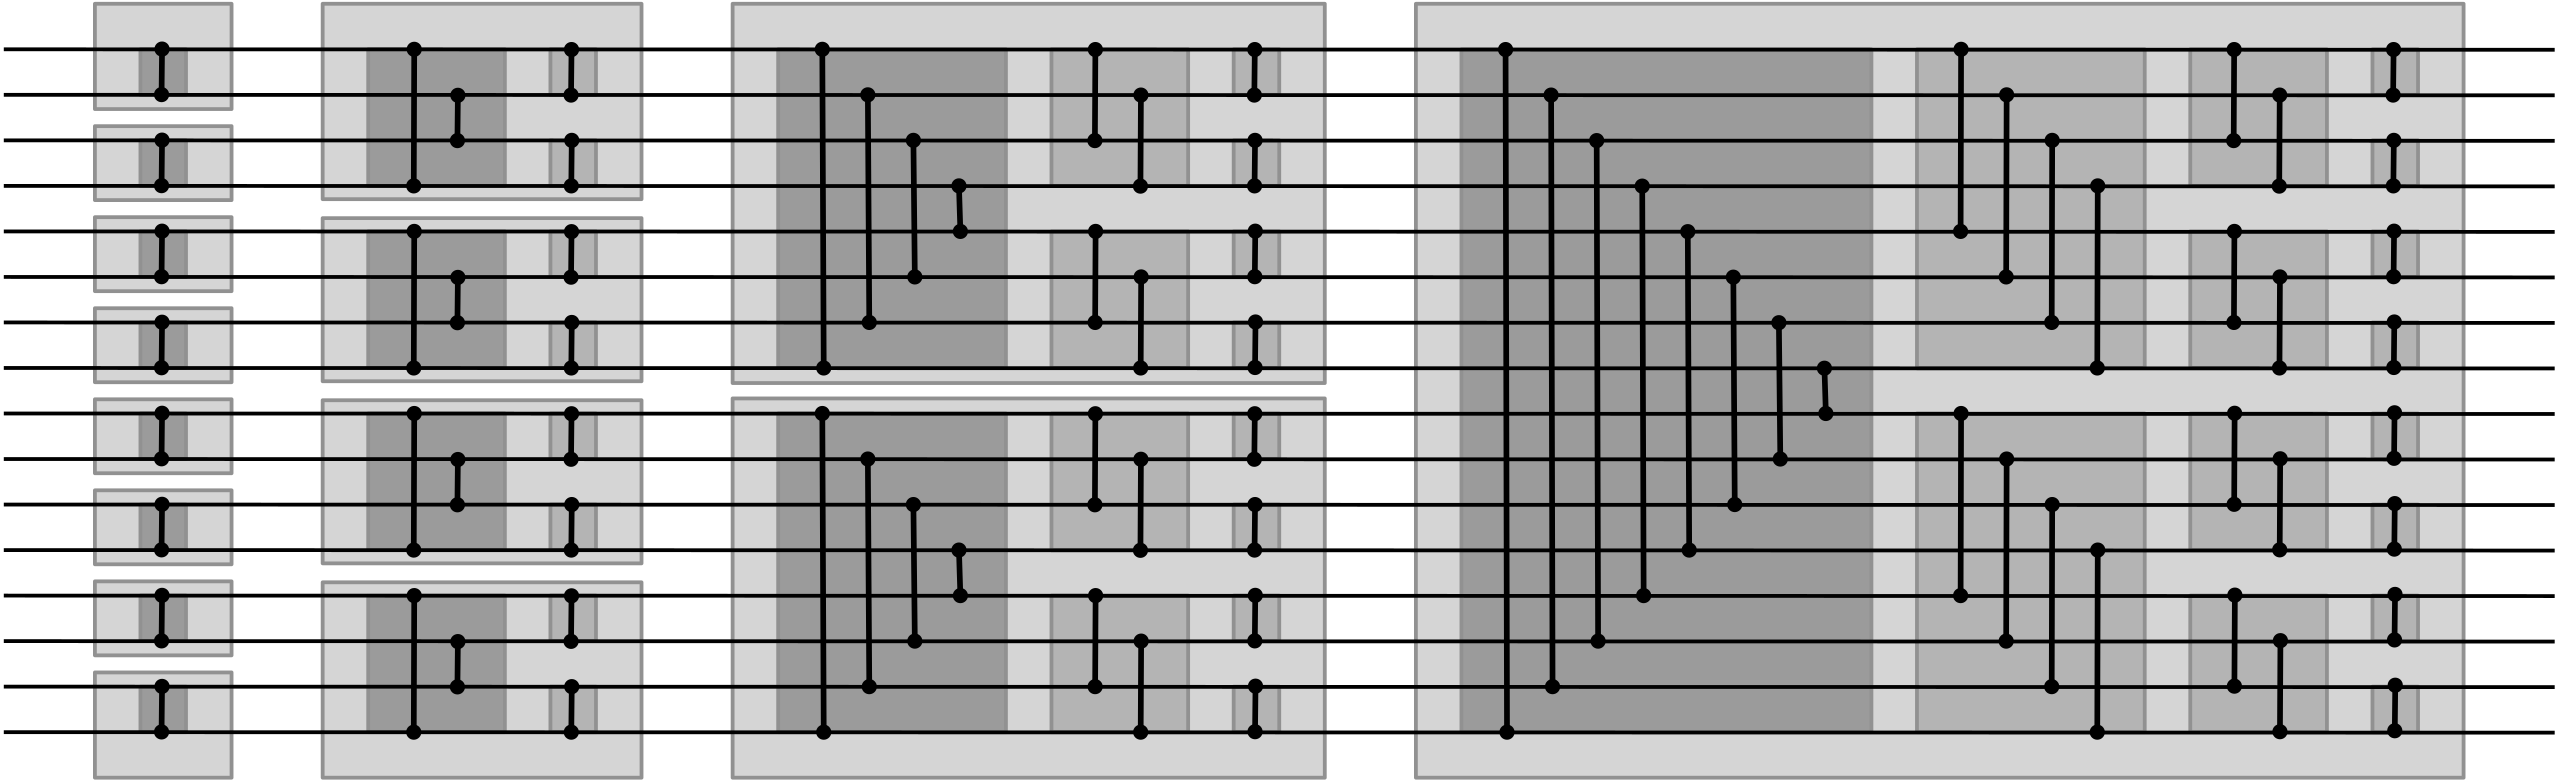
\includegraphics[width=\textwidth]{figures/bitonic-sort.png}
\caption{Sieć sortowania bitonicznego dla $N=16$: dziesięć przebiegów pogrupowanych
w cztery zewnętrzne etapy ($k=1,2,3,4$). Każdy wiersz odpowiada jednemu elementowi,
każda pionowa kreska --- komparatorowi obsługiwanemu przez osobny wątek GPU;
zagnieżdżone prostokąty zaznaczają granice kolejnych etapów zewnętrznych~\cite{christensen2021bitonic}}
\label{fig:bitonic_network}
\end{figure}

Implementacja na GPU mapuje każdy przebieg na osobne wywołanie potoku obliczeniowego.
Dwa parametry charakteryzujące dany przebieg --- wysokość aktualnego bloku bitonicznego
oraz bieżący krok wewnętrzny --- są przekazywane jako stałe wbudowane
(ang.~\textit{push constants}) bezpośrednio przed wywołaniem shadera; dzięki temu ten sam
skompilowany moduł obsługuje wszystkie sześć przebiegów bez konieczności tworzenia oddzielnych
potoków. Rozmiar grupy roboczej wynosi 256 wątków, a jedno wywołanie shadera pokrywa $256 \cdot 2 = 512$
sortowanych elementów, co dla $N$ cząstek przekłada się na $\lceil N/512 \rceil$ grup
roboczych na przebieg.

Zerowa rozbieżność wątków w połączeniu z prostotą operacji porównaj-i-zamień sprawia,
że sortowanie bitoniczne osiąga wysoką przepustowość dla zbiorów o rozmiarze rzędu
kilkudziesięciu tysięcy elementów --- skali typowej dla symulacji małej i średniej liczby
cząstek. Złożoność $O(N \log^2 N)$ staje się jednak coraz mniej korzystna w miarę wzrostu
$N$, co skłoniło do zbadania alternatywy opartej na zliczaniu, omówionej w kolejnym
podrozdziale.

\subsection{Radix Sort}
\label{subsec:radix}

Radix sort jest algorytmem sortowania przez zliczanie, a nie przez porównywanie, co stanowi
fundamentalną różnicę w stosunku do sortowania bitonicznego. Zamiast parować elementy,
każdy przebieg algorytmu zlicza, ile razy w danych pojawia się każda z $2^b$ możliwych
wartości wybranego $b$-bitowego fragmentu klucza, i na tej podstawie oblicza adresy docelowe
każdego elementu. Przy sortowaniu 32-bitowych kluczy po $b=8$ bitów na raz
($r = 2^8 = 256$ kubełków) potrzebne są dokładnie cztery przebiegi, co daje złożoność
$O(kN)$ przy stałym $k=4$ niezależnym od $N$ --- w praktyce liniowy wzrost kosztu z liczbą
sortowanych elementów~\cite{harada2011introduction}.

Każdy z czterech przebiegów rozkłada się na trzy kolejne shadery obliczeniowe
uruchamiane sekwencyjnie z barierami pamięci GPU między nimi: \textit{zliczanie},
\textit{skan prefiksowy} i \textit{reorganizacja}. Przepływ danych w jednym przebiegu
ilustruje rysunek~\ref{fig:radix_one_pass}.

\begin{figure}[h]
\centering
\begin{tikzpicture}[
  sbox/.style={draw, fill=green!10, rounded corners=3pt,
               minimum width=1.0cm, minimum height=1.2cm,
               font=\scriptsize, align=center},
  kbox/.style={draw, fill=blue!10, rounded corners=3pt,
               minimum width=2.8cm, minimum height=1.2cm,
               font=\scriptsize, align=center},
  dbox/.style={draw, fill=orange!10, rounded corners=3pt,
               minimum width=2.0cm, minimum height=1.2cm,
               font=\scriptsize, align=center},
  arr/.style={->, thick, >=Stealth}
]
  \node[sbox] (inp)  at ( 0.0,  0) {wej-\\[1pt]ście\\$N$ el.};
  \node[kbox] (cnt)  at ( 2.8,  0) {\textbf{zliczanie}\\dispatch $[m,1,1]$\\pam.\ dzielona};
  \node[dbox] (cbuf) at ( 5.9,  0) {liczniki\\$m \times 256$\\kol.-major};
  \node[kbox] (scn)  at ( 8.9,  0) {\textbf{skan}\\dispatch $[1,1,1]$\\Hillis--Steele};
  \node[dbox] (obuf) at (11.9,  0) {przesunięcia\\$m \times 256$\\in-place};
  \node[kbox] (ror)  at ( 8.9, -2.6) {\textbf{reorganizacja}\\dispatch $[m,1,1]$\\scatter};
  \node[sbox] (out)  at ( 5.9, -2.6) {wyj-\\[1pt]ście\\$N$ el.};

  \draw[arr] (inp)  -- (cnt);
  \draw[arr] (cnt)  -- (cbuf);
  \draw[arr] (cbuf) -- (scn);
  \draw[arr] (scn)  -- (obuf);
  \draw[arr] (obuf.south) |- (ror.east);
  \draw[arr] (ror)  -- (out);
\end{tikzpicture}
\caption{Przepływ danych w jednym przebiegu sortowania radix. Shadery zliczania
i reorganizacji uruchamiane są z $m = \lceil N/2048\rceil$ grupami roboczymi;
skan prefiksowy zawsze w pojedynczej grupie roboczej (dispatch $[1,1,1]$)
\newline Źródło: Opracowanie własne na podstawie~\cite{harada2011introduction}}
\label{fig:radix_one_pass}
\end{figure}

Shader \textit{zliczanie} jest wywoływany z $m = \lceil N/2048 \rceil$ grupami roboczymi,
gdzie każda przetwarza dokładnie $256 \times 8 = 2048$ elementów --- wynik przyjętego
rozmiaru grupy roboczej wynoszącego 256 wątków przy ośmiu elementach na wątek (stała
\texttt{ELEMENTS\_PER\_INVOCATION}). Każdy wątek wyodrębnia $b$-bitową cyfrę radix z
każdego ze swoich ośmiu elementów przez przesunięcie bitowe i maskowanie, a następnie
zlicza jej wystąpienia operacją atomową \texttt{atomicAdd} na tablicy
\texttt{local\_counts[256]} przechowywanej w pamięci dzielonej grupy roboczej. Koszt
operacji atomowej na pamięci dzielonej jest wielokrotnie niższy niż na pamięci globalnej
GPU --- bez tego kroku wszystkie wątki wszystkich grup roboczych konkurowałyby o te same
256 globalnych liczników, co skutkowałoby serializacją i niwelowałoby zyski z równoległości.
Po przetworzeniu całego segmentu bariera synchronizuje lokalne liczniki w obrębie grupy,
a jeden wątek zapisuje 256 wartości do globalnego bufora liczników pod indeksem
$d \cdot m + \mathrm{wg}$, gdzie $d$ to wartość cyfry radix, a $\mathrm{wg}$ --- numer
grupy roboczej. Ten kolumnowy układ bufora jest nieprzypadkowy: podczas skanowania
kolejne wątki odczytują wartości tego samego kubełka $d$ z kolejnych segmentów pod
kolejnymi adresami pamięci, co zapewnia koalescencję dostępów do pamięci globalnej.

Shader \textit{skan prefiksowy} wywoływany jest zawsze jako pojedyncza grupa robocza
o rozmiarze 256 wątków (dispatch $[1,1,1]$), niezależnie od liczności $N$. Jedna grupa
przekształca tablicę $m \times 256$ liczników w tablicę globalnych przesunięć metodą
Hillisa--Steele'a~\cite{harada2011introduction} w trzech fazach: najpierw obliczana jest
wyłączna suma prefiksowa w obrębie każdego wiersza tablicy, dając lokalne przesunięcia
wewnątrz grupy roboczej; następnie przeprowadzana jest włączna suma prefiksowa po
sumarycznych zliczeniach każdego kubełka; na końcu globalne przesunięcia bloków są
dodawane z powrotem, kompletując tablicę adresów docelowych. Wybór pojedynczej grupy
roboczej eliminuje konieczność wielopoziomowej synchronizacji globalnej, która byłaby
niezbędna przy wielogrupowym skanowaniu --- jest to możliwe właśnie dlatego, że liczba
kubełków wynosi 256, co odpowiada typowej szerokości SIMD architektury GPU i mieści się
w jednej grupie roboczej.

Shader \textit{reorganizacja} przywraca pełny paralelizm: wywoływany z $m$ grupami
roboczymi przetwarzającymi po 2048 elementów każda. Dla każdego elementu wątek oblicza
adres docelowy jako sumę globalnego przesunięcia odczytanego z tablicy przesunięć oraz
lokalnego indeksu tego elementu w obrębie grupy roboczej i kubełka, po czym zapisuje
go pod ten adres w buforze wyjściowym. Operacja ta jest stabilnym scatterem ---
zachowuje wzajemną kolejność elementów o tej samej wartości cyfry radix, co jest
warunkiem koniecznym poprawności całego algorytmu: przebiegi od najmniej znaczących
bitów (ang.~\textit{LSB first}) ku najbardziej znaczącym zachowują poprawną kolejność
z poprzednich przebiegów wyłącznie wtedy, gdy każdy bieżący przebieg jest stabilny.

Implementacja korzysta z dwóch buforów sortowania: głównego \texttt{grid\_entries}
oraz pomocniczego \texttt{entries\_tmp}, wewnętrznego do struktury \texttt{RadixSorter}.
Parzyste przebiegi (0 i~2) kierują dane z \texttt{grid\_entries} do \texttt{entries\_tmp},
nieparzyste (1 i~3) --- w odwrotnym kierunku; po czterech przebiegach wynik jest zawsze
z powrotem w \texttt{grid\_entries}. Złożoność $O(kN)$ ze stałym $k=4$
sprawia, że koszt sortowania rośnie liniowo z liczbą cząstek, co czyni radix sort
algorytmem z wyboru dla dużych symulacji, gdzie logarytmiczne czynniki sortowania
bitonicznego stają się odczuwalne.

\subsection{Porównanie algorytmów}
\label{subsec:sort_comparison}

Mając zaimplementowane oba algorytmy sortowania, można je porównać
zarówno pod kątem właściwości strukturalnych, jak i rzeczywistej wydajności
na GPU. Tabela~\ref{tab:sort_comparison} zestawia najważniejsze cechy obu
metod, podkreślając te różnice, które bezpośrednio wpływają na koszt
wykonania w potoku obliczeniowym.

\begin{table}[htbp]
\centering
\caption{Porównanie własności sortowania bitonicznego i radix}
\label{tab:sort_comparison}
\begin{tabular}{p{4.5cm}p{4.5cm}p{4.5cm}}
\toprule
\textbf{Cecha} & \textbf{Bitonic sort} & \textbf{Radix sort} \\
\midrule
Złożoność czasowa & $O(N \log^2 N)$ & $O(kN)$, $k=4$ \\[3pt]
Liczba dispatchów dla $N=2^{15}$ & 120 & 12 \\[3pt]
Rozbieżność wątków & Zerowa & Zerowa \\[3pt]
Pamięć pomocnicza & Brak (sort. w miejscu) & Bufor \texttt{entries\_tmp} ($8N$~B) i bufor liczników \\[3pt]
Stabilność sortowania & Niestabilna & Stabilna \\[3pt]
Wymóg na $N$ & Potęga dwójki & Dowolne \\
\bottomrule
\end{tabular}
\end{table}

Bezpośredni pomiar czasu sortowania w funkcji liczby elementów $N$
przeprowadzono w środowisku testowym opartym na bezokienkowym kontekście
Vulkan, z buforem wypełnianym pseudolosowymi kluczami
przed każdym uruchomieniem. Czas dla każdego punktu pomiaru wyznaczono jako
medianę z piętnastu niezależnych przebiegów, poprzedzonych trzema przebiegami
rozgrzewkowymi pokrywającymi koszt kompilacji shaderów przez sterownik.
Wyniki, dla $N$ rosnącego od $2^{10}$ do $2^{22}$, przedstawia
rysunek~\ref{fig:sort_benchmark}.

\begin{figure}[H]
\centering
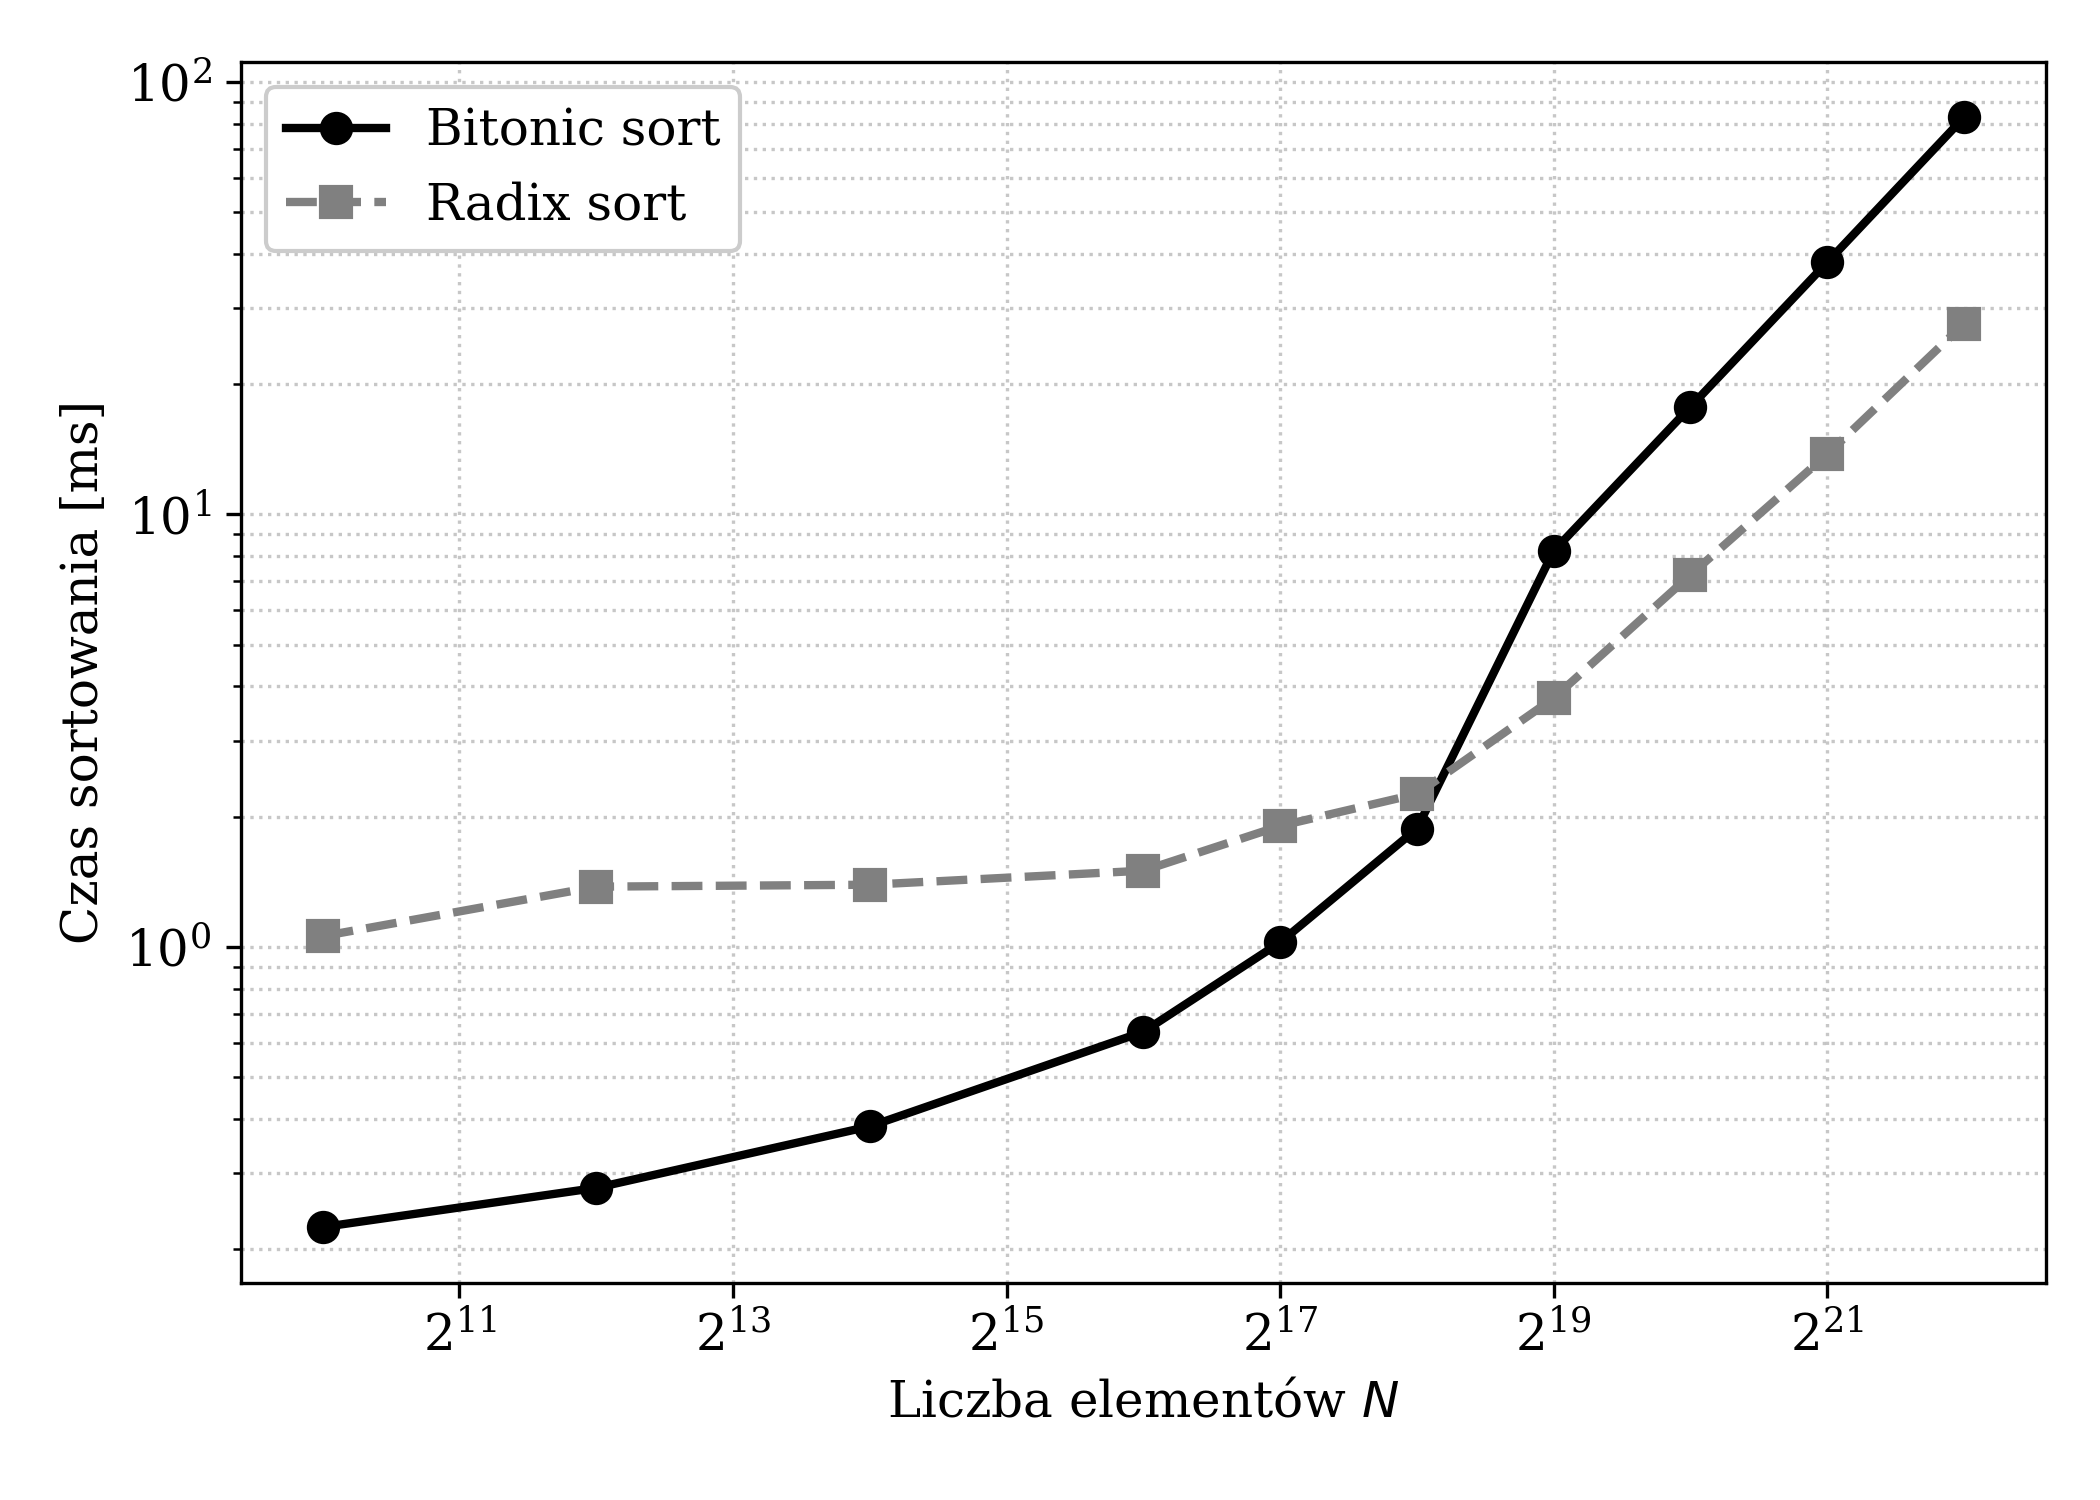
\includegraphics[width=0.85\textwidth]{figures/sort_benchmark.png}
\caption{Czas sortowania bufora \texttt{grid\_entries} jako funkcja liczby
elementów $N$, w skali logarytmicznej na obu osiach. Punkty odpowiadają
medianie z piętnastu przebiegów dla danego $N$
\newline Źródło: Opracowanie własne}
\label{fig:sort_benchmark}
\end{figure}

Dla małej liczby elementów ($N \lesssim 2^{18}$) sortowanie bitoniczne jest
szybsze mimo asymptotycznie gorszej złożoności. Wynika to z bardzo niskiego
stałego narzutu pojedynczego komparatora: każdy przebieg bitoniczny składa się
wyłącznie z odczytu pary elementów, porównania i warunkowej zamiany, podczas
gdy każdy przebieg radix wymaga trzech kolejnych dispatchów ze wzajemną
synchronizacją barierami pamięci. Przy $N \le 2^{14}$ cała praca obliczeniowa
sortowania mieści się w czasie porównywalnym z kosztem wprowadzenia poleceń
do kolejki GPU --- pomiar jest zdominowany przez ten stały narzut, a różnica
między algorytmami pochodzi głównie z liczby dispatchów składowych.

Punkt równowagi obserwuje się między $N = 2^{18}$ a $N = 2^{19}$. Powyżej tego
progu logarytmiczny czynnik bitonicznego $O(N \log^2 N)$ zaczyna dominować nad
stałą liczbą dwunastu dispatchów radix. Dla $N = 2^{22}$ (ponad cztery miliony
elementów) sortowanie radix jest niemal trzykrotnie szybsze: $30{,}5$~ms
względem $82{,}6$~ms dla bitonicznego.

Pomiar wyizolowanego sortowania nie odzwierciedla jednak w pełni zachowania
algorytmu w pełnym potoku obliczeniowym, w którym dispatche sortowania są
przeplatane innymi etapami solvera DFSPH wraz z wymaganymi między nimi
barierami pamięci. Profil Tracy zarejestrowany dla symulacji z 25\,000 cząstek
(rysunki~\ref{fig:tracy_bitonic} i~\ref{fig:tracy_radix}) pokazuje, że średni
czas wykonania etapu \texttt{neighbor\_search\_post\_integrate} ---
obejmującego haszowanie, sortowanie, wyznaczenie przesunięć i reorganizację
buforów --- wynosi $3{,}64$~ms dla wariantu bitonicznego i $616{,}3$~µs
dla wariantu radix. Oba pomiary dotyczą tej samej konfiguracji symulacji,
więc niemal sześciokrotna różnica wynika wyłącznie z wyboru algorytmu
sortowania.

\begin{figure}[htbp]
\centering
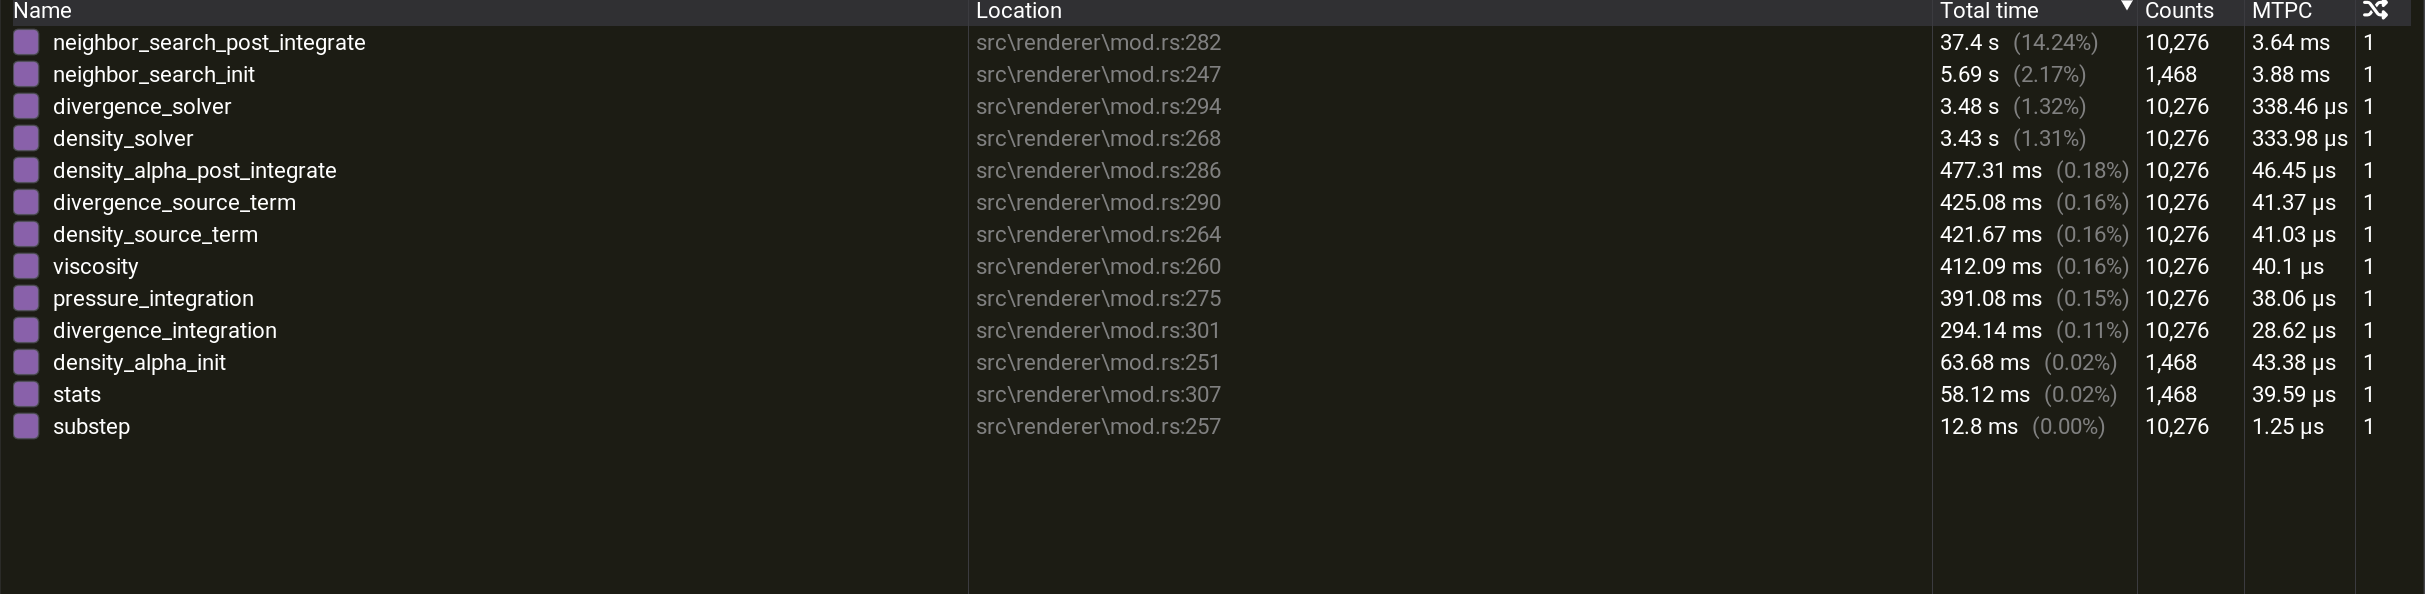
\includegraphics[width=0.95\textwidth]{figures/bitonic_tracy_profile.png}
\caption{Profil Tracy dla wariantu z sortowaniem bitonicznym, $N=25\,000$
cząstek. Wiersz \texttt{neighbor\_search\_post\_integrate} pokazuje średni
czas $3{,}64$~ms na wywołanie
\newline Źródło: Opracowanie własne}
\label{fig:tracy_bitonic}
\end{figure}

\begin{figure}[htbp]
\centering
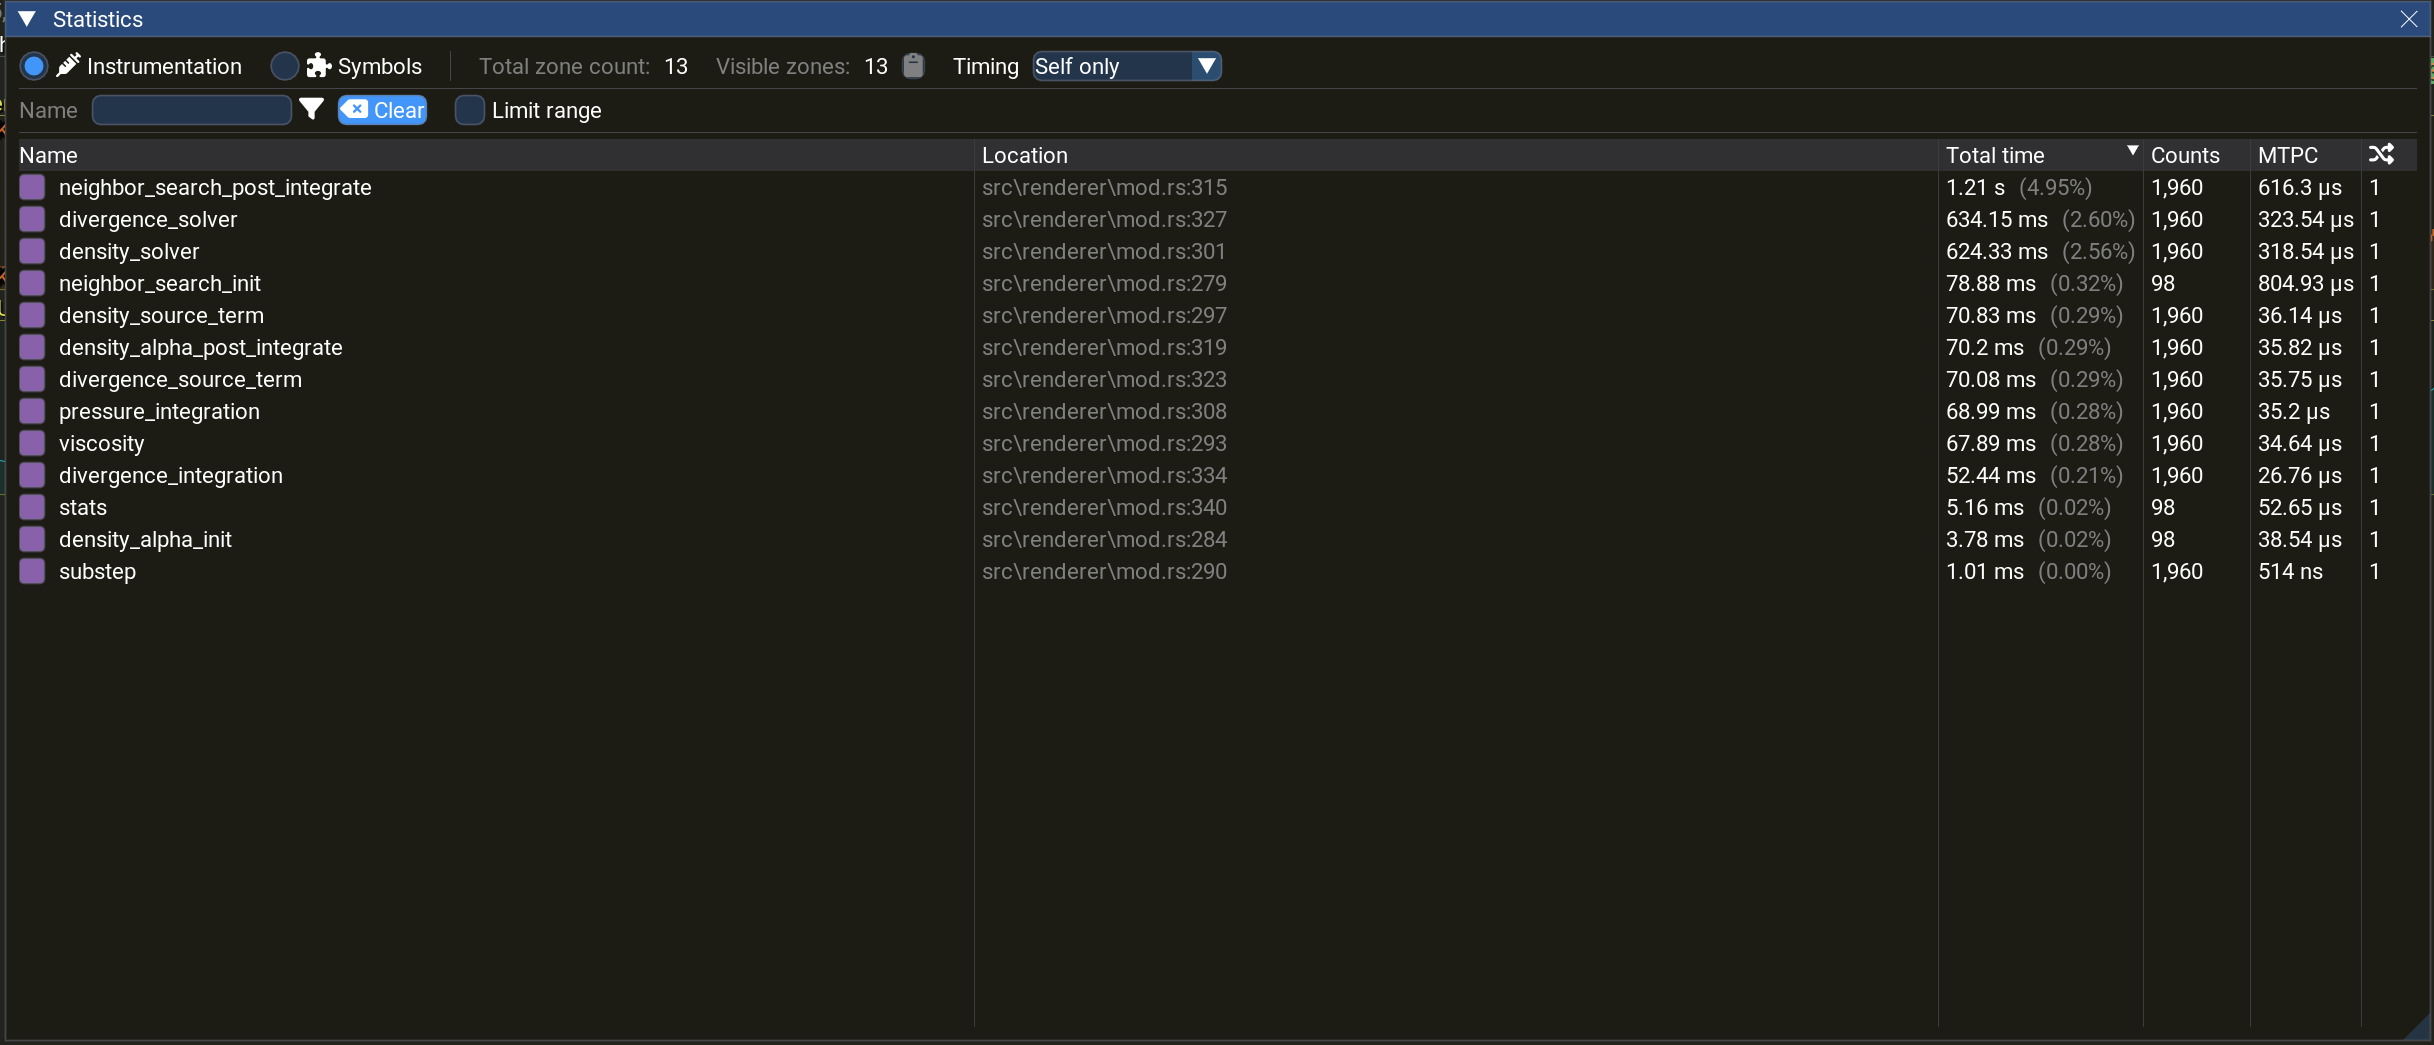
\includegraphics[width=0.95\textwidth]{figures/radix_tracy_profile.png}
\caption{Profil Tracy dla wariantu z sortowaniem radix w tym samym
scenariuszu. Średni czas tego samego zakresu spada do $616{,}3$~µs
\newline Źródło: Opracowanie własne}
\label{fig:tracy_radix}
\end{figure}

Rozbieżność między izolowanym testem porównawczym (gdzie radix dla $N = 2^{15}$ jest
nieznacznie wolniejszy) a pomiarem produkcyjnym (gdzie ten sam $N$ daje
sześciokrotne przyspieszenie) ma uzasadnienie strukturalne. Sortowanie
bitoniczne $32\,768$ elementów ($\lceil 25\,000 \rceil_2$) wymaga
$\frac{\log_2^2 32768 + \log_2 32768}{2} = 120$ dispatchów, z których każdy
w pełnym potoku jest oddzielony od kolejnego barierą pamięci wstawioną przez
\texttt{AutoCommandBufferBuilder}; radix wymaga ich jedynie dwunastu. W teście
izolowanym, gdzie GPU wykonuje wyłącznie sortowanie, koszt pojedynczej bariery
jest amortyzowany przez wysoką zajętość jednostek obliczeniowych. W pełnym
potoku DFSPH bariera staje się jawnym punktem synchronizacji, ponieważ
poprzedza ją zapis innego shadera obliczeniowego --- a sumaryczny koszt skaluje
się z liczbą dispatchów algorytmu sortowania.

Łączny obraz prowadzi do jednoznacznego wyboru: dla każdego rozmiaru symulacji
od kilku tysięcy cząstek wzwyż radix sort jest szybszym wariantem, a jego
przewaga rośnie zarówno z $N$, jak i z liczbą innych etapów obliczeniowych
dzielących GPU. Sortowanie bitoniczne pozostaje w kodzie jako alternatywa
dostępna do przełączenia w czasie wykonania przez wariant
\texttt{SortAlgorithm::Bitonic}, użyteczna w celach porównawczych oraz
w scenariuszach, w których prostota sieci komparatorów ma znaczenie większe
niż mierzona wydajność.

% ------------------------------------------------------------
\section{Solver DFSPH}
\label{sec:dfsph}

Wszystkie wcześniejsze sekcje tej części pracy --- organizacja pamięci
w układzie SOA z parami buforów dla pozycji i prędkości, haszowanie
przestrzenne wraz z sortowaniem i reorganizacją buforów oraz autorska
cecha \texttt{ComputeStep} unifikująca cykl życia potoków obliczeniowych
--- istnieją wyłącznie po to, by w tym miejscu mogła zostać zrealizowana
sama symulacja dynamiki cieczy. Dyskretyzacja jądrowa metody SPH
wprowadzona w podrozdziale~\ref{subsec:kernel-interpolation},
dwuetapowa korekcja DFSPH zdefiniowana algorytmami~\ref{alg:density_source}
i~\ref{alg:div_source} oraz konkretne struktury danych z sekcji~\ref{sec:data_structures}
zbiegają się tutaj w jeden spójny potok obliczeniowy. Każdy z jego etapów
jest osobnym implementatorem cechy \texttt{ComputeStep} i odpowiada
konkretnemu fragmentowi matematycznego sformułowania metody; ich kolejność
oraz wzajemne zależności określają, w jaki sposób abstrakcyjne równania
teoretyczne odwzorowują się na rzeczywiste shadery obliczeniowe wykonywane
na GPU.

Z implementacyjnego punktu widzenia kluczowa jest asymetria między obydwoma
poziomami korekcji: \textit{korekcja gęstości} kończy się adwekcją pozycji
$\mathbf{p}_i \leftarrow \mathbf{p}_i + \Delta t\,\mathbf{v}_i$,
natomiast \textit{korekcja dywergencji} działa wyłącznie na buforze
prędkości i nie modyfikuje pozycji cząstek.
Ta różnica determinuje kolejność shaderów w pętli substepów.
Poza nią oba poziomy współdzielą identyczną strukturę: iteracyjna pętla
ciśnienia z tym samym wzorcem dostępu do sąsiedztwa, różniąca się
wyłącznie wyrazem źródłowym i finalnym krokiem integracji.

Wszystkie shadery realizujące fizykę SPH dzielą jeden fundamentalny wzorzec
dostępu do danych. Niezależnie od tego, czy obliczają gęstość, wyraz
źródłowy, siłę ciśnienia czy korekcję lepkościową, każdy z nich akumuluje
sumę po geometrycznym sąsiedztwie cząstki~$i$, ważoną jądrem~$W$ lub jego
gradientem~$\nabla W$. Konkretna postać akumulowanej wielkości różni się
między etapami, lecz struktura pętli pozostaje niezmiennikiem całego potoku.
Wykorzystując bufor \texttt{grid\_start} przygotowany przez potok
wyszukiwania sąsiadów (sekcja~\ref{sec:neighbor_search}), każdy shader
wyznacza komórkę przestrzenną swojej cząstki i iteruje po
$3 \times 3 \times 3 = 27$ komórkach sąsiednich, używając ich skrótów jako
indeksów wejścia do listy posortowanych wpisów.
Jądro $W(\|\mathbf{r}\|, h)$ zwraca skalarną wagę, malejącą z odległością;
jego gradient $\nabla W(\mathbf{r}, h)$ jest wektorem wskazującym kierunek
i tempo zmian tej wagi.
W obliczeniach SPH $W$ pojawia się wszędzie tam, gdzie sumujemy wielkości
skalarne --- jak gęstość --- natomiast $\nabla W$ wszędzie tam, gdzie
potrzebna jest siła lub przyspieszenie.
Algorytm~\ref{alg:neighbor_iter} przedstawia ten uniwersalny wzorzec.

\begin{algorithm}[htbp]
\caption{Wspólny wzorzec iteracji po sąsiadach w shaderach SPH}
\label{alg:neighbor_iter}
$\mathbf{c}_i \leftarrow \lfloor \mathbf{p}_i / h \rfloor$\;
\For{$dz \in \{-1,\,0,\,+1\}$}{
  \For{$dy \in \{-1,\,0,\,+1\}$}{
    \For{$dx \in \{-1,\,0,\,+1\}$}{
      $k \leftarrow \mathrm{hash}(\mathbf{c}_i + (dx, dy, dz))$\;
      $s \leftarrow \texttt{grid\_start}[k]$\;
      \While{$s < M$ \upshape \textnormal{i} $\texttt{grid\_entries}[s].\texttt{hash} = k$}{
        $j \leftarrow \texttt{grid\_entries}[s].\texttt{index}$\;
        $\mathbf{r}_{ij} \leftarrow \mathbf{p}_i - \mathbf{p}_j$\;
        \If{$\|\mathbf{r}_{ij}\| < h$}{
          akumulacja wkładu pary $(i, j)$ z wagą $W(\|\mathbf{r}_{ij}\|,\,h)$ lub $\nabla W(\mathbf{r}_{ij},\,h)$\;
        }
        $s \leftarrow s + 1$\;
      }
    }
  }
}
\end{algorithm}

Identyczna pętla iteracji po sąsiadach występuje we wszystkich shaderach solvera DFSPH
--- różni je wyłącznie wyrażenie pod sumą
oraz atrybut, do którego trafia wynik akumulacji. Dzięki przepisaniu pozycji
i prędkości na bufory \texttt{\_b} przez etap \texttt{reorder}
(\ref{subsec:neighbor_pipeline}), kolejne wpisy danej komórki leżą gęsto
w pamięci, a odczyt całego 27-elementowego sąsiedztwa wykonuje się
w niewielkiej liczbie skoalescowanych transakcji pamięci globalnej GPU.

Tabela~\ref{tab:dfsph_variable_mapping} odwzorowuje wielkości figurujące
w sformułowaniu matematycznym DFSPH na konkretne bufory struktury
\texttt{GpuPhysicsData} oraz na shadery odpowiedzialne za ich zapis.
Ze względu na podwójne buforowanie cząstek (\ref{subsec:gpu_buffers}),
pozycje i prędkości występują w dwóch wariantach: bufor \texttt{\_a}
przechowuje stabilny stan wejściowy, na podstawie którego haszowanie
przestrzenne wyznacza komórki cząstek; bufor \texttt{\_b}, do którego
\texttt{reorder} przepisuje dane w kolejności sprzyjającej lokalności
odczytu, stanowi wejście dla wszystkich kolejnych etapów solvera.
Pozostałe wielkości to jednowymiarowe tablice indeksowane numerem cząstki.

\begin{table}[H]
\centering
\caption{Odwzorowanie wielkości teoretycznych DFSPH na bufory GPU}
\label{tab:dfsph_variable_mapping}
\begin{tabular}{p{4.8cm}p{4.5cm}p{4.5cm}}
\toprule
\textbf{Wielkość} & \textbf{Bufor} & \textbf{Etap zapisujący} \\
\midrule
$\mathbf{p}_i$ --- pozycja                  & \texttt{position\_a}, \texttt{position\_b}    & \texttt{reorder}, \texttt{pressure\_integration} \\[3pt]
$\mathbf{v}_i$ --- prędkość                 & \texttt{velocity\_a}, \texttt{velocity\_b}    & \texttt{reorder}, \texttt{viscosity}, korekcje ciśnienia \\[3pt]
$\rho_i$ --- gęstość                        & \texttt{densities}                            & \texttt{density\_alpha} \\[3pt]
$\alpha_i$ --- współczynnik DFSPH           & \texttt{factors}                              & \texttt{density\_alpha} \\[3pt]
$s_i$ --- wyraz źródłowy                    & \texttt{source\_terms}                        & \texttt{density\_source\_term}, \texttt{divergence\_source\_term} \\[3pt]
$p_i$ --- ciśnienie                         & \texttt{pressures}                            & \texttt{pressure\_update} \\[3pt]
$\mathbf{a}_i^{p}$ --- przysp. ciśnienia    & \texttt{pressure\_accelerations}              & \texttt{pressure\_force} \\
\bottomrule
\end{tabular}
\end{table}

Pozostałe podrozdziały tej sekcji szczegółowo omawiają poszczególne
komponenty solvera. Podrozdział~\ref{subsec:substep_loop} przedstawia
pełną pętlę substepów ustalającą kolejność wszystkich etapów wewnątrz
pojedynczej klatki. Podrozdział~\ref{subsec:density} opisuje obliczanie
gęstości $\rho_i$ oraz współczynnika $\alpha_i$, pełniącego rolę
prekondycjonera w solverze ciśnienia.
Podrozdziały~\ref{subsec:density_correction}
i~\ref{subsec:divergence_correction} analizują kolejno korekcję gęstości
i korekcję dywergencji --- dwie iteracyjne pętle ciśnienia, które łącznie
wymuszają nieściśliwość pola prędkości. Podrozdział~\ref{subsec:cfl}
omawia warunek CFL i strategię doboru kroku czasowego $\Delta t$.

\subsection{Pętla substepów}
\label{subsec:substep_loop}

Pełna sekwencja wywołań shaderów w obrębie substepu ukazana jest
w Algorytmie~\ref{alg:frame_loop}.
Bezpośrednio po adwekcji następuje przebudowa struktury wyszukiwania
sąsiadów. To drugie wywołanie \texttt{neighbor\_search} w obrębie jednego
substepu nie jest redundancją --- jest koniecznością wynikającą z fizycznego
przemieszczenia cząstek.
Tablica \texttt{grid\_start}, zbudowana przed substepem, indeksuje pozycje
sprzed adwekcji; korekcja dywergencji oparta na nieaktualnej strukturze
obliczałaby gradient prędkości $\nabla \cdot \mathbf{v}$ względem błędnych
sąsiadów, co prowadziłoby do narastających błędów kompresji szczególnie
widocznych przy dużych prędkościach cząstek.
Po przebudowie sąsiedztwa i ponownym wyznaczeniu $\rho_i$, $\alpha_i$
faza dywergencji przebiega analogicznie: iteracyjna pętla $N_\nabla$ razy
uruchamia ten sam \texttt{pressure\_force} i \texttt{pressure\_update}
z wyrazem źródłowym opartym na dywergencji pola prędkości,
po czym \texttt{divergence\_integration} aktualizuje prędkości
bez modyfikowania pozycji.

Iteracyjny charakter obu solwerów wynika z natury problemu.
Zmiana ciśnienia cząstki~$i$ generuje przyspieszenie oddziałujące na
jej sąsiadów, które z kolei wymagają korekty swoich ciśnień ---
i tak dalej.
Jedno przejście pętli realizuje krok analogiczny do iteracji Jacobiego:
wyznacza lokalną poprawkę przy założeniu, że ciśnienia sąsiadów pozostają
chwilowo zamrożone.
Kilka takich kroków ($N_\rho = 2$--$5$, $N_\nabla = 1$--$3$)
zazwyczaj wystarcza do sprowadzenia średniego błędu poniżej zadanego progu;
strategię doboru tych liczb omówiono w podrozdziale~\ref{subsec:cfl}.

\subsection{Obliczanie gęstości}
\label{subsec:density}

Szader \texttt{density\_and\_alpha} oblicza w jednym przebiegu dwie
wielkości: gęstość $\rho_i$ oraz współczynnik $\alpha_i$~\cite{bender2015divergence}.
Listing~\ref{lst:density_alpha} przedstawia funkcję \texttt{main()} shadera.

\begin{lstlisting}[caption={Szader \texttt{density\_and\_alpha} --- logika akumulacji},
                   label=lst:density_alpha,]
void main() {
    uint i = gl_GlobalInvocationID.x;
    if (i >= uint(positions.length())) return;

    float density     = 0.0;
    float sum_grad_sq = 0.0;
    vec3  grad_sum    = vec3(0.0);

    // iteracja po 27 sąsiednich komórkach
    float r = sqrt(dot(r_vec, r_vec));
    density += mass * kernel_w(r, h);
    if (r > 1e-6) {
        vec3 mass_grad  = mass * kernel_grad(r_vec, r, h);
        grad_sum       += mass_grad;
        sum_grad_sq    += dot(mass_grad, mass_grad);
    }
    // koniec petli

    densities[i] = density;
    float alpha = sum_grad_sq + dot(grad_sum, grad_sum);
    if (alpha > 1e-6) { factors[i] = alpha; }
    else              { factors[i] = 0.0;   }
}
\end{lstlisting}

Każda invokacja odpowiada jednej cząstce~$i$.
Zmienna \texttt{density} akumuluje skalarne wkłady jądra \texttt{kernel\_w}
po 27 sąsiednich komórkach --- jest to bezpośrednia realizacja wzorca
z Algorytmu~\ref{alg:neighbor_iter}.
Zmienne \texttt{grad\_sum} i \texttt{sum\_grad\_sq} akumulują jednocześnie
składniki współczynnika $\alpha_i$: odpowiednio sumę gradientów
$\sum_j m\nabla W_{ij}$ oraz sumę ich kwadratów $\sum_j |m\nabla W_{ij}|^2$;
wynikowe $\alpha_i = |\texttt{grad\_sum}|^2 + \texttt{sum\_grad\_sq}$
stanowi mianownik korekcji ciśnienia w każdym kroku iteracyjnym solvera.
Obliczenie obu wielkości w jednej pętli zamiast dwóch oddzielnych
przebiegów redukuje o połowę liczbę odczytów z pamięci globalnej GPU.



\subsection{Korekcja gęstości}
\label{subsec:density_correction}

Faza korekcji gęstości wymusza nieściśliwość, wyznaczając ciśnienia redukujące 
odchylenia $\rho_i$ od wartości docelowej $\rho_0$.
Szader \texttt{density\_source\_term} oblicza dla każdej cząstki~$i$
człon źródłowy łączący chwilowy deficyt gęstości z prognozą jego narastania
na podstawie prędkości adwekcyjnych wyznaczonych po fazie lepkości:

\begin{lstlisting}[caption={Szader \texttt{density\_source\_term} --- człon źródłowy solvera gęstości},
                   label=lst:density_source,]
float divergence_sum = 0.0;
// dla kazdego sasiada j w promieniu h:
vec3 vel_diff = vel_i - vel_j;
divergence_sum += mass * dot(vel_diff, grad);
// koniec petli

float source = ((rho_0 - rho_i) / dt) - divergence_sum;
source_terms[i] = source;
pressures[i] = 0.0;
\end{lstlisting}

Składnik \texttt{(rho\_0 - rho\_i) / dt} mierzy bieżący błąd gęstości 
skalowany krokiem czasowym; \texttt{divergence\_sum} aproksymuje metodą SPH dywergencję 
pola prędkości adwekcyjnych, przewidując jak ten błąd będzie dalej narastał. 
Tablica \texttt{pressures} jest zerowana na wejściu każdego wywołania,
gwarantując start iteracji ze świeżym wektorem ciśnień.

Iteracja Jacobiego przebiega przez naprzemienne wywołania \texttt{pressure\_force} i \texttt{pressure\_update}. 
Pierwszy szader wyznacza dla każdej cząstki przyspieszenie ciśnieniowe
będące iloczynem macierzy układu i wektora ciśnień; drugi aktualizuje ciśnienie:

\begin{lstlisting}[caption={Szader \texttt{pressure\_update} --- krok Jacobiego},
                   label=lst:pressure_update,]
float a_ii       = -(dt / (rho_i * rho_i)) * alpha_i;
float error      = source_i - Ap_i;
float correction = (relax_factor * error) / a_ii;
pressures[i]     = max(p_i + correction, 0.0);
\end{lstlisting}

Zmienna \texttt{a\_ii} to przekątny element operatora ciśnieniowego 
obliczony bezpośrednio z $\alpha_i$ wyznaczonego przez \texttt{density\_and\_alpha}; 
\texttt{relax\_factor} ($\omega = 0{,}5$) ogranicza oscylacje typowe dla niezrelaksowanej iteracji 
Jacobiego. Wywołanie \texttt{max(\ldots, 0.0)} 
eliminuje ujemne ciśnienia: bez niego cząstki przy swobodnej
powierzchni, których gęstość spełnia $\rho_i < \rho_0$, generowałyby siły
przyciągające, prowadząc do niestabilności tensylnej.

Test \texttt{rest\_density\_diagnostic} ujawnił 
wyraźną dwumodalność rozkładu gęstości (Rys.~\ref{fig:rest_density}): 
cząstki wewnętrzne osiągają $\rho_i \approx \rho_0$, natomiast cząstki przy swobodnej 
powierzchni wykazują systematyczny deficyt wynikający z niepełnej sumy jądra SPH. 
Właśnie ten deficyt powoduje plateau widoczne w teście zbieżności (Rys.~\ref{fig:convergence}, panel lewy) --- błąd $\overline{|\rho_i - \rho_0|}$ 
utrzymuje się na poziomie $\sim\!200~\mathrm{kg/m^3}$ niezależnie od liczby iteracji, 
ponieważ solver poprawnie zeruje ciśnienie dla pod-gęstych cząstek brzegowych, 
nie próbując korygować efektu wynikającego z geometrii.
Właściwa obsługa brzegu za pomocą cząstek-duchów~\cite{schechter2012ghost} wykracza poza zakres niniejszej pracy.

\begin{figure}[htbp]
    \centering
    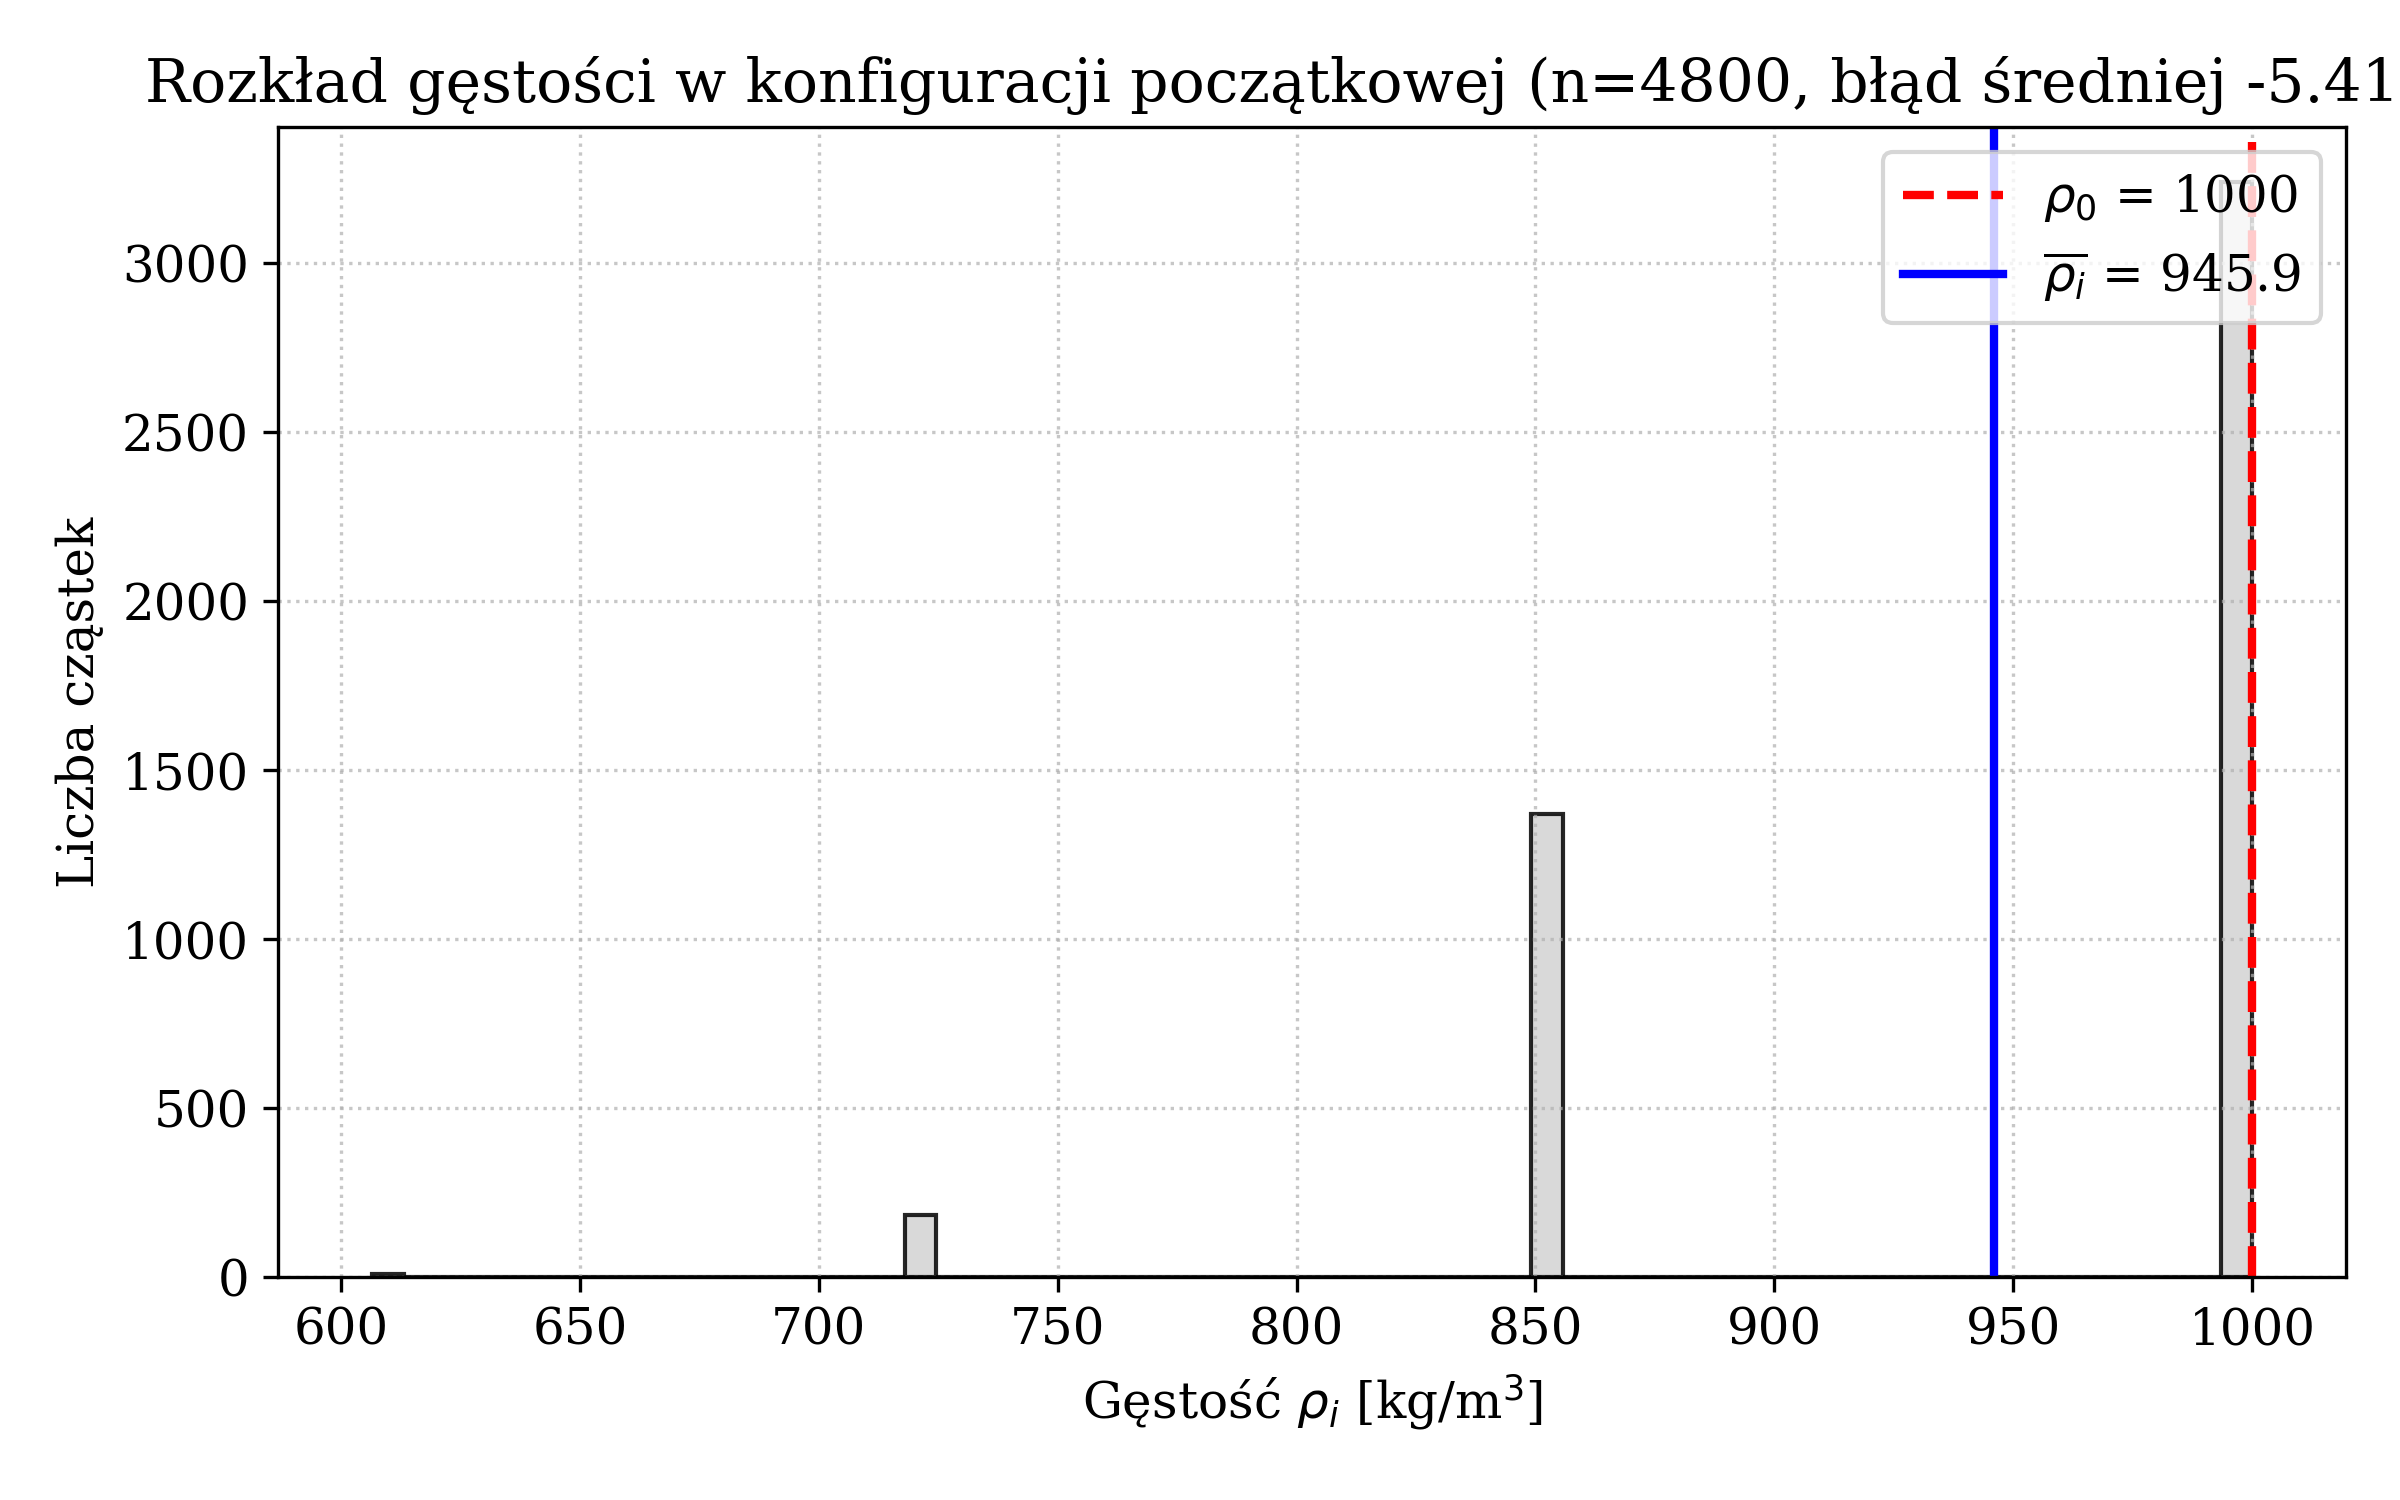
\includegraphics[width=0.85\linewidth]{figures/rest_density.png}
    \caption{Histogram gęstości w konfiguracji spoczynkowej ($n = 4800$ cząstek, bez kroku symulacji). Cząstki wewnętrzne skupiają się przy $\rho_0 = 1000~\mathrm{kg/m^3}$; cząstki przy swobodnej powierzchni wykazują deficyt będący ograniczeniem standardowego SPH bez obsługi brzegu. Źródło: opracowanie własne}
    \label{fig:rest_density}
\end{figure}

\subsection{Korekcja dywergencji}
\label{subsec:divergence_correction}

Faza korekcji dywergencji działa na prędkościach cząstek po przesunięciu ich przez solver gęstości.
Jej celem jest wyzerowanie dywergencji pola prędkości $\nabla \cdot \mathbf{v} = 0$, eliminując pozostałą składową kompresji.
Szader \texttt{divergence\_source\_term} oblicza człon źródłowy z prędkości bezpośrednio po całkowaniu ciśnień:

\begin{lstlisting}[caption={Szader \texttt{divergence\_source\_term} --- człon źródłowy solvera dywergencji},
                   label=lst:divergence_source,]
float divergence_sum = 0.0;
// dla kazdego sasiada j w promieniu h:
vec3 vel_diff = vel_i - vel_j;
divergence_sum += mass * dot(vel_diff, grad);
// koniec petli

source_terms[i] = -divergence_sum;
\end{lstlisting}

W odróżnieniu od solvera gęstości, człon źródłowy nie zawiera składnika $(\rho_0 - \rho_i)/\Delta t$ --- celem jest wyłącznie zerowanie dywergencji.
Pętla Jacobiego jest identyczna (\texttt{pressure\_force} i \texttt{pressure\_update}), natomiast szader \texttt{divergence\_integration} stosuje wynikowe ciśnienia jako korekty prędkości, nie pozycji:

\begin{lstlisting}[caption={Szader \texttt{divergence\_integration} --- całkowanie prędkości},
                   label=lst:divergence_integration,]
vec3 new_vel = vel + ap * dt;
velocities[i] = vec4(new_vel, 0.0);
\end{lstlisting}

Prawy panel Rys.~\ref{fig:convergence} ujawnia odwrotną zależność:
błąd dywergencji wzrasta wraz z liczbą iteracji i formuje symetryczne plateau od góry.
Jest to bezpośrednie sprzężenie z solverem gęstości: jedna iteracja ledwo koryguje gęstość
i nieznacznie przesuwa cząstki, pozostawiając pole prędkości prawie bezrozbieżne;
dwie i więcej iteracji skutecznie redukuje $\rho_i - \rho_0$ drogą dużych przesunięć,
które indukują proporcjonalnie silniejszą dywergencję prędkości.
Oba wykresy tworzą zatem lustrzany obraz: plateau błędu gęstości od dołu
odpowiada plateau błędu dywergencji od góry, wyznaczonemu przez skalę przesunięć
generowanych przez solver gęstości w stanie nasycenia.
Ponieważ błąd gęstości nigdy nie spada do zera z powodu deficytu jądra na brzegu,
solver gęstości stale generuje impulsy ciśnieniowe, a solver dywergencji nie ma szans
ustabilizować pola prędkości --- stąd trwałe plateau po obu stronach wykresu.

\begin{figure}[htbp]
    \centering
    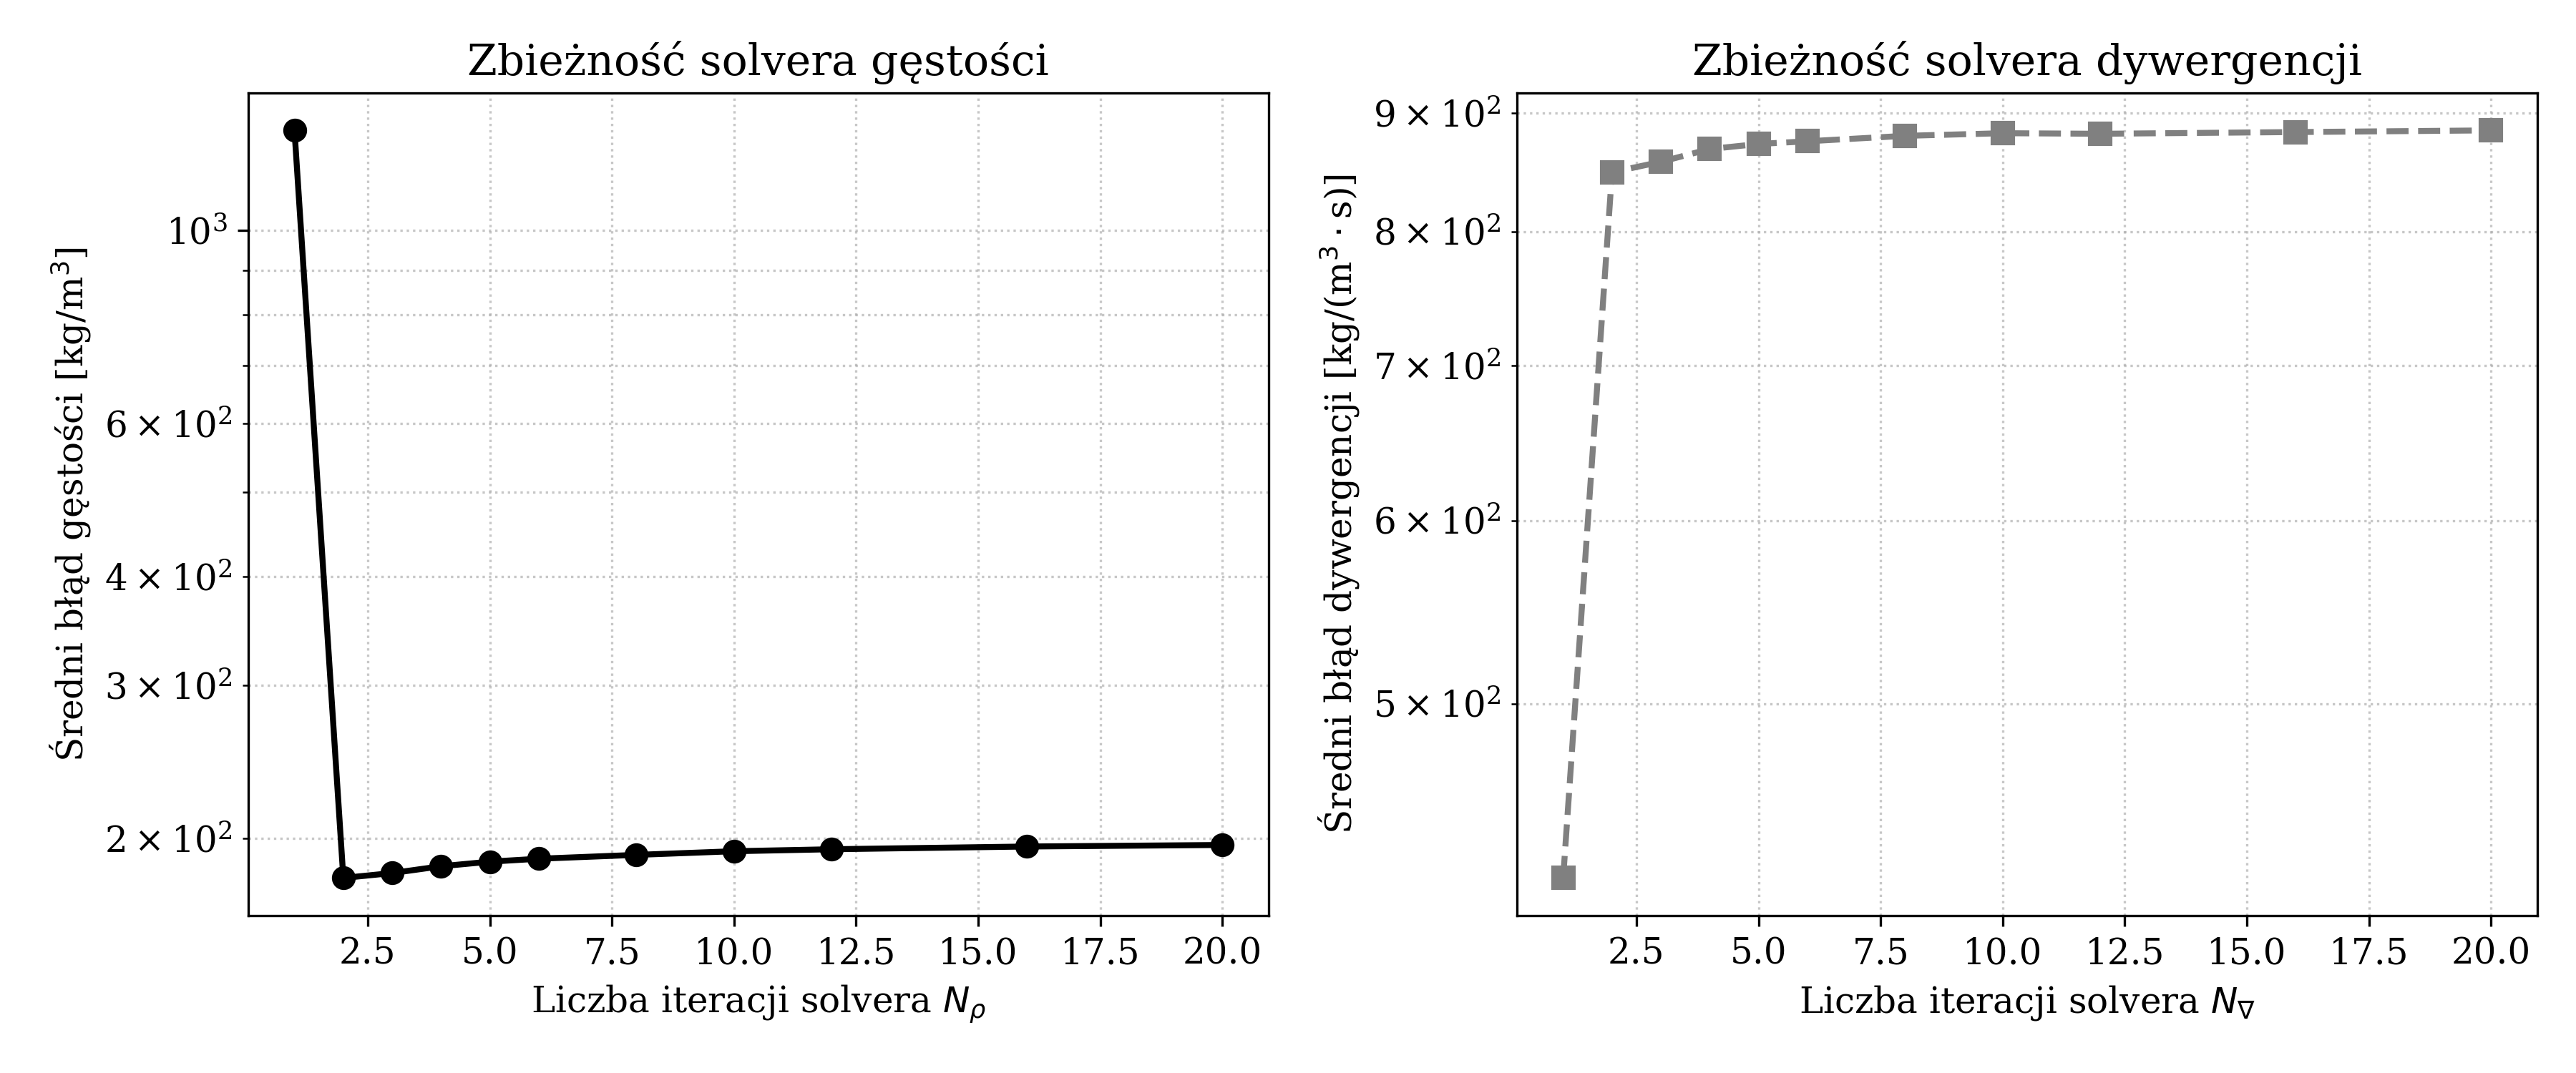
\includegraphics[width=\linewidth]{figures/convergence.png}
    \caption{Zbieżność solvera DFSPH: uśredniony błąd gęstości (lewy panel) i błąd dywergencji (prawy panel) w funkcji liczby iteracji Jacobiego. Każdy punkt to uśrednienie 40~kroków symulacji po 50~krokach rozgrzewki ($n = 4800$ cząstek). Plateau błędu gęstości wynika z deficytu jądra SPH na brzegu; plateau błędu dywergencji wynika ze sprzężenia z solverem gęstości. Źródło: opracowanie własne}
    \label{fig:convergence}
\end{figure}

\subsection{Warunek CFL i dobór \(\Delta t\)}
\label{subsec:cfl}

Dobór kroku czasowego $\Delta t$ kształtował się przez kilka etapów prób i korekt,
z których każdy ujawniał kolejną warstwę ograniczeń implementacji.

\paragraph{Etap 1 --- stały \(\Delta t\) i stała liczba iteracji.}
Pierwsza wersja symulatora operowała stałym krokiem $\Delta t = 5~\mathrm{ms}$
i czterema iteracjami Jacobiego per solver per krok symulacji.
Wynik był akceptowalny: symulacja przebiegała stabilnie przez większość czasu,
lecz sporadycznie załamywała się wskutek kumulacji błędu numerycznego.
Niska liczba klatek na sekundę skłoniła do poszukiwania optymalizacji.

\paragraph{Etap 2 --- adaptacyjny \(\Delta t\) według warunku CFL.}
Warunek CFL ogranicza krok czasowy tak,
aby cząstka nie przemieściła się o więcej niż jeden promień wygładzania $h$:
\begin{equation}
  \Delta t \leq \lambda \frac{h}{v_{\max}},
  \label{eq:cfl}
\end{equation}
gdzie $\lambda < 1$ to współczynnik bezpieczeństwa, a $v_{\max}$ to chwilowa prędkość
maksymalna odczytywana z bufora statystyk GPU (\texttt{stats\_buffer[0]}).
Gdy symulacja uspokaja się i $v_{\max}$ maleje, $\Delta t$ może wzrosnąć,
co bezpośrednio przekłada się na wyższą liczbę klatek na sekundę.
Pojawił się jednak nowy problem: większy $\Delta t$ powoduje szybsze narastanie błędu
gęstości, przez co cztery iteracje Jacobiego okazały się niewystarczające.

\paragraph{Etap 3 --- kryterium zatrzymania oparte na progu błędu.}
Naturalnym rozwinięciem było dodanie drugiego warunku zakończenia iteracji:
kontynuuj, dopóki $\overline{|\rho_i - \rho_0|} > \varepsilon$.
W założeniu solver miał wykonywać 4--5 iteracji przy spokojnej symulacji
i więcej przy gwałtownych ruchach, a rosnące $\Delta t$ kompensowało koszt
dodatkowych iteracji.
W praktyce każdy solver wykonywał sto iteracji (skonfigurowane maksimum) i nigdy
nie osiągał progu zbieżności.
Przyczyna jest dokładnie tą, którą ujawnił test zbieżności
(podrozdz.~\ref{subsec:density_correction}): deficyt jądra SPH na swobodnej
powierzchni trwale blokuje błąd gęstości na poziomie $\sim\!200~\mathrm{kg/m^3}$,
niezależnie od liczby iteracji.
Nawet milion iteracji nie obniżyłby go poniżej żadnego sensownego progu.

\paragraph{Decyzja końcowa.}
Jako kompromis powrócono do stałego $\Delta t = 5~\mathrm{ms}$ i stałej liczby
czterech iteracji per solver.
Rozwiązanie zapewnia przewidywalny koszt obliczeniowy klatki i eliminuje ryzyko
zawieszenia symulatora w nieskończonej pętli iteracyjnej.
Utrzymują się dwa znane ograniczenia: niska liczba klatek na sekundę wynikająca
z braku adaptacji kroku oraz ryzyko niestabilności numerycznej przy długich sesjach.
Oba są bezpośrednią konsekwencją braku właściwej obsługi brzegu ---
bez niej kryterium $\varepsilon$-zbieżności nie może działać poprawnie.

\begin{figure}[htbp]
  \centering
  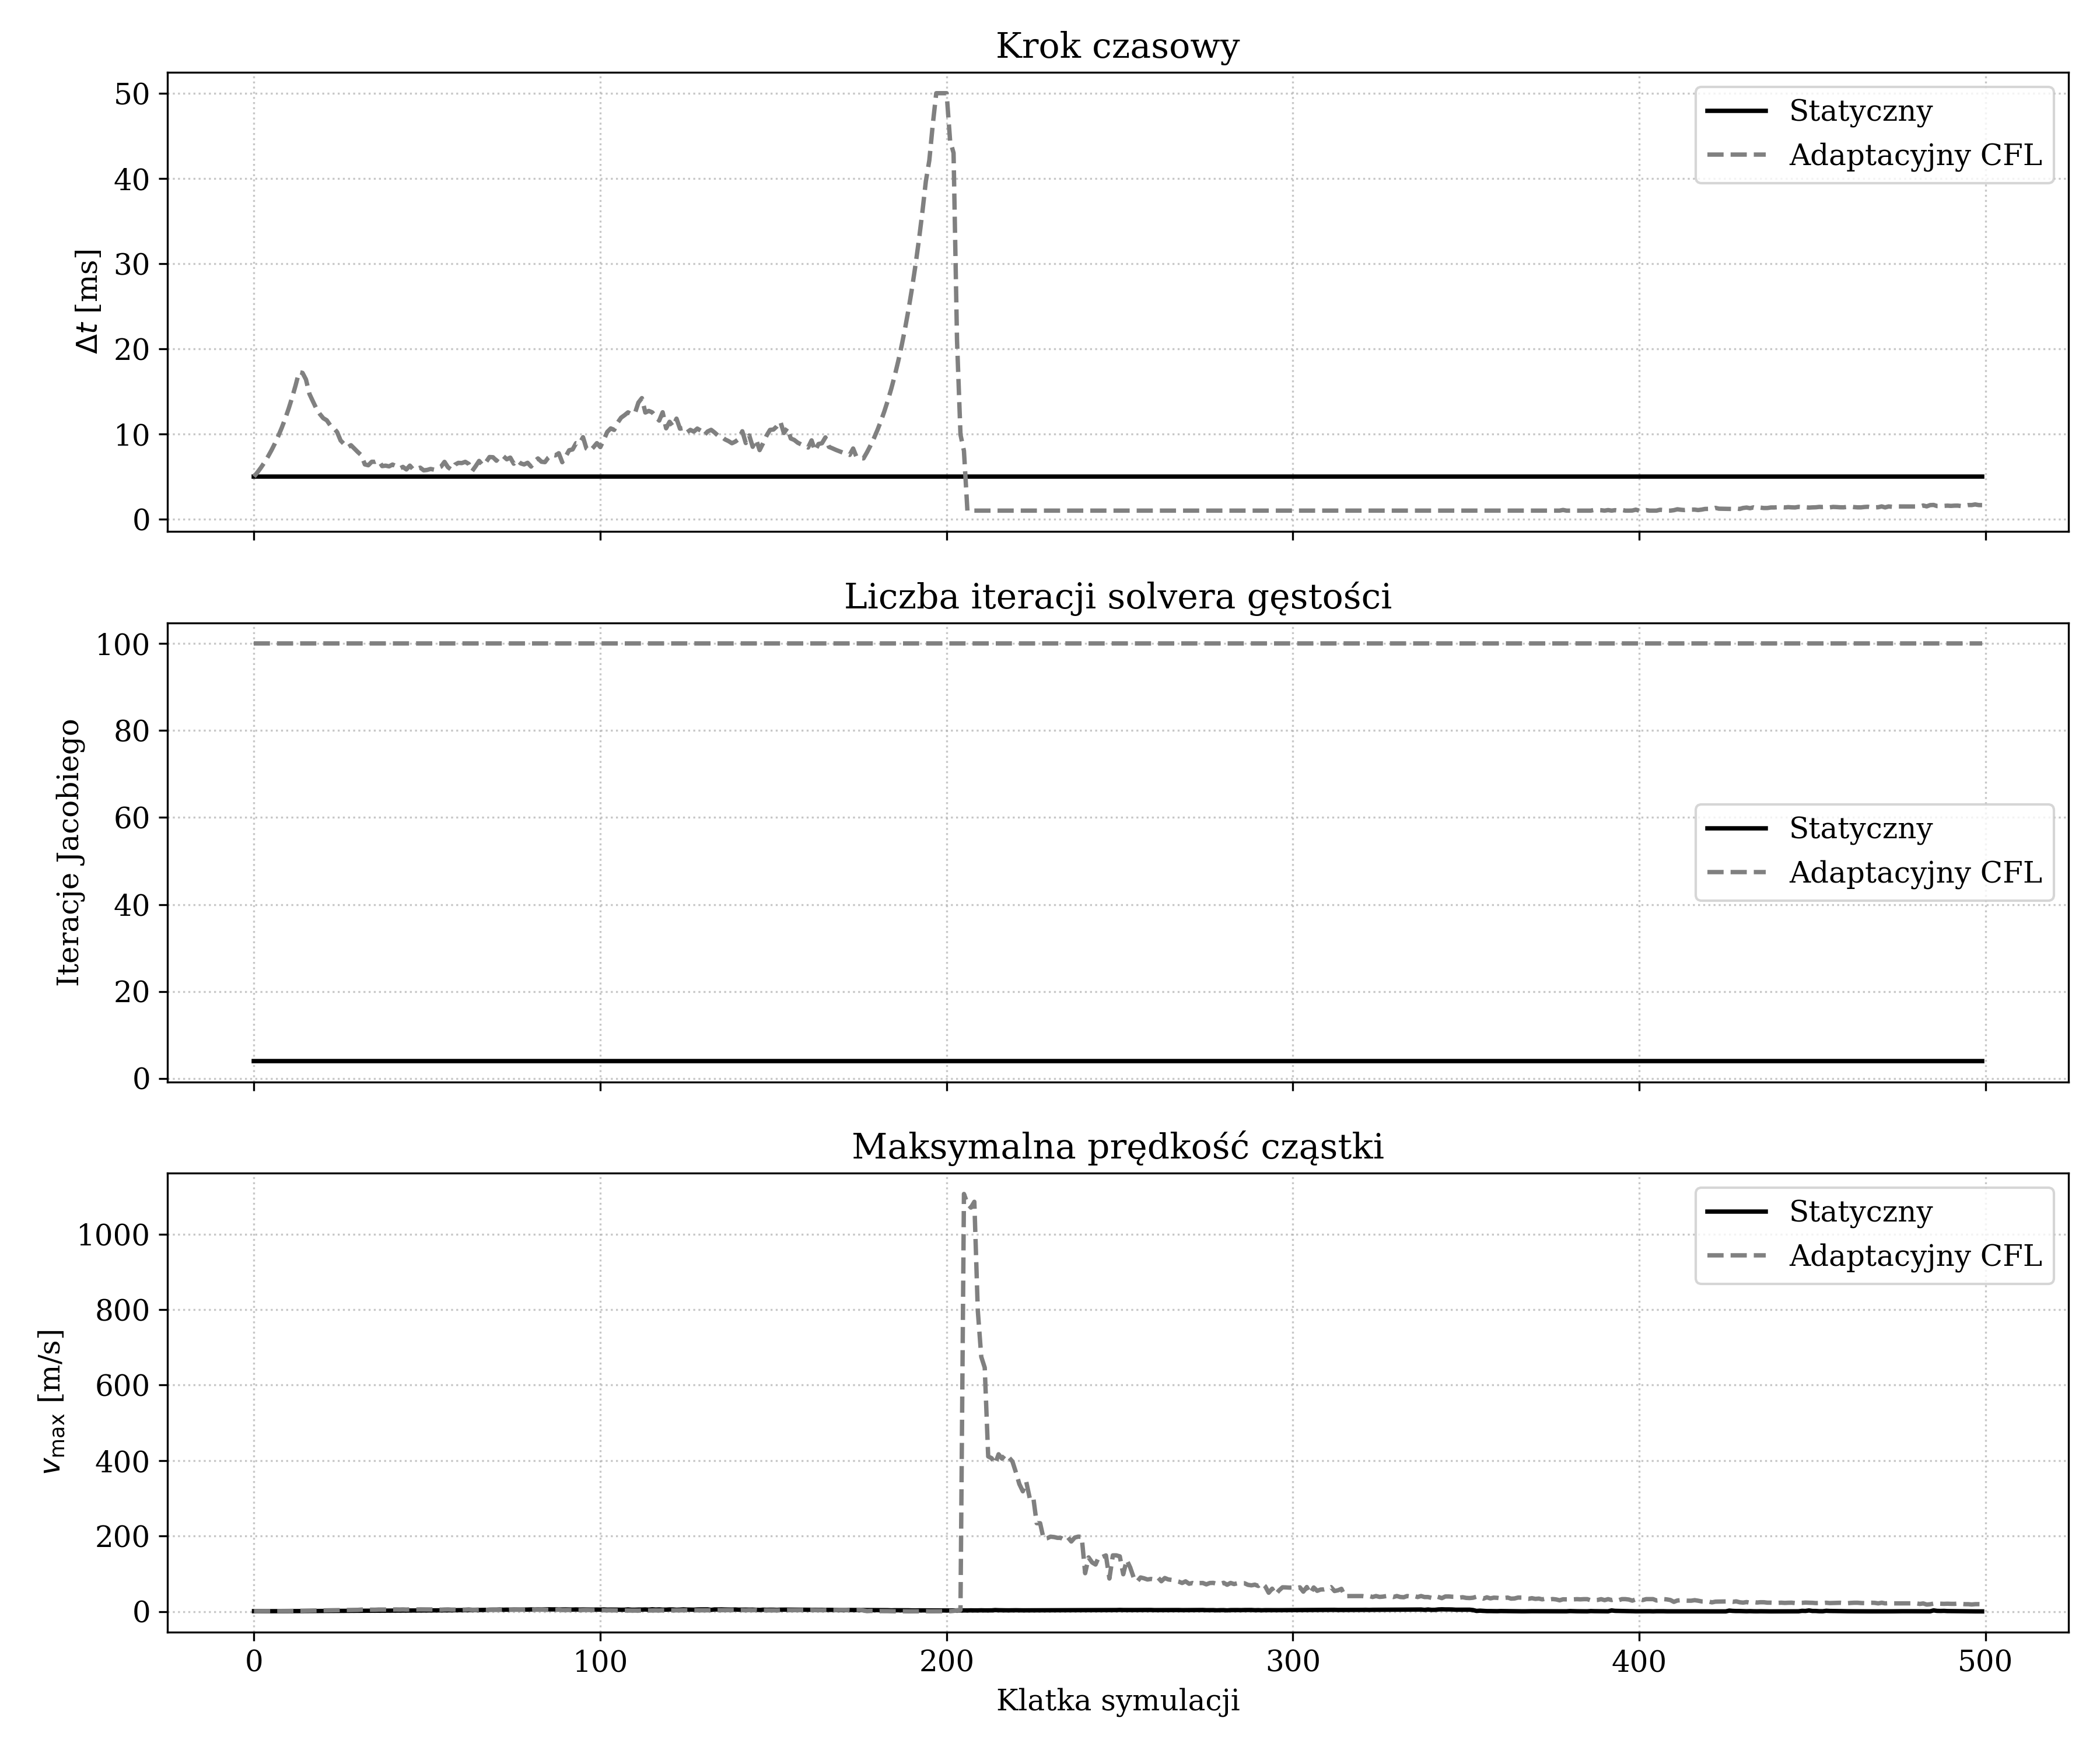
\includegraphics[width=\textwidth]{figures/cfl_comparison.png}
  \caption{Porównanie strategii statycznego $\Delta t$ (linia ciągła) i adaptacyjnego
    $\Delta t$ według warunku CFL (linia przerywana) w trakcie 500 klatek symulacji.
    \textbf{Górny panel:} krok czasowy $\Delta t$ w milisekundach.
    Wariant statyczny utrzymuje stałe $5~\mathrm{ms}$; wariant adaptacyjny rośnie
    do $50~\mathrm{ms}$ w chwilach spokoju cieczy, po czym w okolicach klatki~205
    wywołuje katastrofalną niestabilność ($v_{\max} \approx 1100~\mathrm{m/s}$)
    i opada do minimalnego $1~\mathrm{ms}$.
    \textbf{Środkowy panel:} liczba iteracji solvera Jacobiego.
    Wariant statyczny utrzymuje stałe cztery iteracje; wariant adaptacyjny
    osiąga limit 100 iteracji w każdej klatce bez wyjątku, ponieważ próg
    $\varepsilon$ nigdy nie jest spełniony.
    \textbf{Dolny panel:} maksymalna prędkość cząstki $v_{\max}$.
    Po eksplozji prędkość stabilizuje się na poziomie $20$--$40~\mathrm{m/s}$,
    co wskazuje na stan uszkodzonej symulacji.\\
    Źródło: opracowanie własne}
  \label{fig:cfl_comparison}
\end{figure}

% ------------------------------------------------------------
\section{Siły fizyczne}
\label{sec:forces}

Podrozdział ten opisuje implementację dwóch mechanizmów siłowych działających
na cząsteczki poza solverem DFSPH: wygładzenia prędkości metodą XSPH oraz
odpowiedzi na kolizje z granicą domeny.
Podstawy teoretyczne obu metod omówiono w podrozdziale~\ref{sec:physical_models_theory};
poniżej skupiono się na konkretnych wyborach implementacyjnych i stałych
liczbowych przyjętych w kodzie.

\subsection{Lepkość XSPH}
\label{subsec:xsph}

Wygładzenie prędkości XSPH realizowane jest w shaderze \texttt{viscosity}.
Poniższy listing przedstawia rdzeń obliczeń --- pętlę po sąsiadach
i końcową aktualizację prędkości:

\begin{lstlisting}[caption={Rdzeń shadera \texttt{viscosity} --- korekcja XSPH i grawitacja},
                   label=lst:xsph,]
vec3 sum_viscosity = vec3(0.0);
// dla kazdego sasiada j w promieniu h:
vec3 vel_diff = velocities[j].xyz - velocities[i].xyz;
sum_viscosity += mass / densities[j] * vel_diff * kernel_w(r, h);
// koniec petli

vec3 vel_visco = velocities[i].xyz
               + sim_params.viscosity * sum_viscosity;
new_velocities[i] = vec4(vel_visco + sim_params.gravity.xyz
                                   * sim_params.dt, 0.0);
\end{lstlisting}

Bezwymiarowy współczynnik wygładzenia $\nu$ przechowywany jest w polu
\texttt{viscosity} struktury \texttt{SimulationParams}.
Wartość $\nu = 0{,}15$ dobrano empirycznie: wartości poniżej $0{,}05$
dopuszczają widoczne przenikanie cząsteczek przy zderzeniach,
powyżej $0{,}4$ nadmiernie tłumią ruch i spowalniają opadanie.
Parametr jest dostępny w czasie wykonania przez suwak interfejsu egui
bez potrzeby ponownej kompilacji shaderów.

Grawitacja dodawana jest w tej samej przepustce tuż po korekcji XSPH,
co eliminuje oddzielny dispatch i jedno przejście przez bufor prędkości.
Wynik trafia do bufora \texttt{new\_velocities}; zapis i odczyt dotyczą
różnych buforów, więc kolejność wątków nie wpływa na wynik.

\subsection{Obsługa kolizji}
\label{subsec:collision}

Reakcja na kolizję z ścianą odbywa się na końcu shadera
\texttt{pressure\_integration}, bezpośrednio po całkowaniu Eulera.
Listing~\ref{lst:collision} pokazuje obsługę jednej ściany (dolna granica
osi~$y$); pozostałe pięć ścian realizowane są analogicznie:

\begin{lstlisting}[caption={Fragment \texttt{pressure\_integration} --- odbicie od dolnej sciany},
                   label=lst:collision,]
float restitution = 0.5;
float friction    = 0.95;
float eps         = 0.001;

if (new_pos.y < min_b.y + r) {
    new_pos.y  = min_b.y + r + eps;
    new_vel.y *= -restitution;
    new_vel.xz *= friction;
}
\end{lstlisting}

Stała \texttt{eps} przesuwa cząsteczkę o $1~\mathrm{mm}$ ponad granicę,
zapobiegając wielokrotnemu wyzwalaniu warunku w kolejnych krokach.
Współczynnik sprężystości $e = 0{,}5$ pochłania połowę energii normalnej
przy każdym odbiciu; tarcie styczne $f = 0{,}95$ nieznacznie tłumi
ruch równoległy do ściany, nie zatrzymując cząsteczki całkowicie.

Podejście to nie koryguje deficytu jądra przy brzegu omówionego
w~podrozdz.~\ref{subsec:divergence_correction}, lecz skutecznie
zapobiega ucieczce cząsteczek z domeny i jest wystarczające dla
wizualnie wiarygodnych scen zamkniętych.

% ------------------------------------------------------------
\section{Wizualizacja}
\label{sec:visualization}

Potok wizualizacji przekształca listę pozycji cząsteczek w gotowy kolor piksela
w trzech etapach: splatowanie gęstości do trójwymiarowej tekstury, przemarsz promienia
przez tę teksturę do znalezienia powierzchni, oraz model optyczny łączący odbicie,
załamanie, absorpcję i rozproszenie podpowierzchniowe.
Podstawy teoretyczne wszystkich etapów omówiono w podrozdziale~\ref{sec:visualization_pipeline_theory};
poniżej przedstawiono konkretne stałe i fragmenty kodu z implementacji.

\subsection{Splatowanie gęstości do tekstury 3D}
\label{subsec:density_splat}

Shader \texttt{splat\_density} dla każdej cząsteczki wyznacza woksel centralny,
a następnie iteruje po sześcianie $\pm 8$ wokseli i atomowo dodaje wkład do tekstury:

\begin{lstlisting}[caption={Shader \texttt{splat\_density} --- waga woksela i zapis atomowy},
                   label=lst:splat,]
int radius = 8;
\ dla kazdego woksela (x,y,z) w szescianie [-radius, radius]^3:
float dist   = length(vec3(x, y, z));
if (dist < float(radius)) {
    float x_norm = dist / float(radius);
    float weight = (1.0 - x_norm * x_norm);
    weight = weight * weight * weight;

    uint contrib = uint(weight * 200.0);
    imageAtomicAdd(density_grid, currentVoxel, contrib);
}
\end{lstlisting}

Waga jest gładkim wielomianem $(1-q^2)^3$ tożsamym z~eq.~\ref{eq:splat_weight}.
Mnożnik $200$ skaluje wartość do zakresu liczby całkowitej bez utraty precyzji;
woksele powietrza osiągają wartości bliskie zeru, woksele wewnątrz cieczy --- rzędu
setek.
Tekstura ma format \texttt{R32Uint}; stała \texttt{DENSITY\_OFFSET = 300} odejmowana
jest przy odczycie w shaderze fragmentów, eliminując szum tła bez progowania binarnego.

\subsection{Ray Marching}
\label{subsec:raymarching}

Pętla przemarszu w \texttt{raymarch} składa się z trzech faz: testu AABB,
grubego kroku oraz bisekcji refinementu.

\paragraph{Test AABB i krok gruby.}
Przed wejściem w pętlę funkcja \texttt{intersectAABB} wyznacza analitycznie
przedział $[t_{\min}, t_{\max}]$ wejścia i wyjścia promienia z domeny;
promienie chybiające domenę odrzucane są natychmiast instrukcją \texttt{discard}.

\begin{lstlisting}[caption={Fragment \texttt{raymarch} --- test AABB i petla przemarszu},
                   label=lst:march_loop,]
const int   MAX_STEPS = 96;
const float STEP_SIZE = 0.007;

vec2 tHit = intersectAABB(rayOrigin, rayDir, boxMin, boxMax);
if (tHit.x > tHit.y || tHit.y < 0.0) discard;

float stepWorld = STEP_SIZE
                * max(max(boxScale.x, boxScale.y), boxScale.z);
float tCurrent  = max(tHit.x, 0.0);

for (int i = 0; i < MAX_STEPS; i++) {
    if (tCurrent > tHit.y) break;
    if (getDensity(rayOrigin + rayDir * tCurrent, ...) > 0.01) {
        hit = true; break;
    }
    tCurrent += stepWorld;
}
if (!hit) discard;
\end{lstlisting}

Krok \texttt{stepWorld} skalowany jest rozmiarem sceny, dzięki czemu ta sama stała
\texttt{STEP\_SIZE} działa poprawnie niezależnie od proporcji domeny.
Promienie, które nie trafią w żaden woksel powyżej progu w 96 krokach, są odrzucane
instrukcją \texttt{discard} jeszcze na etapie shadera fragmentów.

\paragraph{Bisekcja i normalna.}
Po wykryciu pierwszego przekroczenia progu przedział $[t_0, t_1]$ zawężany
jest ośmiokrotną bisekcją, a normalna wyznaczana jest różnicami skończonymi
na polu gęstości.

\begin{lstlisting}[caption={Fragment \texttt{raymarch.frag} --- bisekcja i normalna},
                   label=lst:bisect,]
float t0 = tCurrent - stepWorld, t1 = tCurrent;
for (int i = 0; i < 8; i++) {
    float m = (t0 + t1) * 0.5;
    if (getDensity(rayOrigin + rayDir * m, ...) > 0.01)
        t1 = m;
    else
        t0 = m;
}
vec3 surfacePos = rayOrigin + rayDir * t1;
vec3 N = -calcNormal(surfacePos, boxMin, boxMax);
if (dot(N, N) < 0.5) N = vec3(0.0, 1.0, 0.0);
\end{lstlisting}

Osiem iteracji bisekcji zawęża punkt trafiania do dokładności
$\Delta t / 2^8 \approx 0{,}4\%$ kroku bez zmniejszania globalnego
\texttt{STEP\_SIZE}.
Normalna wyznaczana jest sześcioma próbkami pola gęstości metodą różnic skończonych
(\texttt{eps = 0.018}); warunek \texttt{dot(N,N) < 0.5} zastępuje normalną wektorem
pionowym w miejscach, gdzie gradient zanika (płaskie dno).

\paragraph{Interpolacja trójliniowa.}
Próbkowanie tekstury \texttt{R32Uint} realizowane jest ręcznie, ponieważ format
całkowitoliczbowy nie obsługuje sprzętowej interpolacji:

\begin{lstlisting}[caption={Funkcja \texttt{getDensity} --- interpolacja trojliniowa},
                   label=lst:trilinear,]
vec3 gridPos = uvw * vec3(sim_params.grid_res.xyz) - 0.5;
ivec3 iobase = ivec3(floor(gridPos));
vec3  f      = fract(gridPos);
\ 8 wywolan texelFetch dla wierzcholkow kostki (v000..v111)
float v0 = mix(mix(v000, v100, f.x), mix(v010, v110, f.x), f.y);
float v1 = mix(mix(v001, v101, f.x), mix(v011, v111, f.x), f.y);
return max(0.0, (mix(v0, v1, f.z) - DENSITY_OFFSET) 
                    * DENSITY_MULTIPLIER);
\end{lstlisting}

Odjęcie \texttt{DENSITY\_OFFSET = 300} zeruje szum tła; \texttt{max(0.0, ...)}
zapobiega ujemnym wartościom gęstości w wokselach powietrza.

\subsection{Model oświetlenia}
\label{subsec:shading}

Cały model optyczny zamknięty jest w funkcji \texttt{main()} shadera
\texttt{raymarch.frag} i wykonywany po znalezieniu punktu powierzchni.

\paragraph{Fresnel, odbicie i załamanie.}
Współczynnik odbicia $F_0$ wyznaczany jest ze wzoru Fresnela, a promienie
odbitego i załamanego kierunku próbkują skybox:

\begin{lstlisting}[caption={Fragment \texttt{raymarch.frag} --- Fresnel, odbicie, zalamania},
                   label=lst:fresnel,]
const float IOR_WATER = 1.333;
const float IOR_AIR   = 1.0;

float F0 = pow((IOR_AIR - IOR_WATER) / (IOR_AIR + IOR_WATER), 2.0);
float F  = fresnel(NdotV, F0);  // przyblizenie Schlicka

vec3 reflDir    = reflect(rayDir, N);
vec3 reflection = sampleSkybox(reflDir);
reflection += SUN_COLOR * clamp(ggxD(NdotH, 0.04) 
                * NdotL * 0.15, 0.0, 3.0);

vec3 refrDir    = refract(rayDir, N, IOR_AIR / IOR_WATER);
if (dot(refrDir, refrDir) < 0.01) refrDir = rayDir;
vec3 background = sampleSkybox(normalize(refrDir));
\end{lstlisting}

Wartość $F_0 \approx 0{,}02$ obliczana jest ze wzoru Fresnela dla granicy
woda--powietrze; przy kącie ślizgowym wzrasta do jedności zgodnie z przybliżeniem
Schlicka.
W przypadku całkowitego wewnętrznego odbicia \texttt{refract} zwraca wektor zerowy;
kierunek zastępowany jest wówczas oryginalnym promieniem.

\paragraph{Absorpcja, SSS i piana.}
Grubość cieczy wzdłuż promienia steruje absorpcją Beer-Lamberta,
rozproszeniem podpowierzchniowym i maską piany; wynik składany jest
operatorem Reinharda do zakresu $[0,\,1]$:

\begin{lstlisting}[caption={Fragment \texttt{raymarch.frag} --- absorpcja, SSS, piana, tonowanie},
                   label=lst:sss,]
const vec3 ABSORPTION_COEFF = vec3(0.45, 0.085, 0.025);
const vec3 SCATTER_COLOR    = vec3(0.04, 0.18,  0.28);

float thickness  = calcThickness(
    surfacePos, 
    rayDir, 
    tHit.y - t1, ...);
vec3  absorption = exp(-ABSORPTION_COEFF * thickness * 8.0);

float sssWrapped = max(0.0, dot(N,  L) * 0.5 + 0.5);
float sssBack    = max(0.0, dot(-N, L));
float sssFactor  = (sssWrapped * 0.6 + sssBack * 0.4)
                 * (1.0 - exp(-thickness * 3.0));
vec3 sss = SCATTER_COLOR * SUN_COLOR * sssFactor * SCATTER_STRENGTH;

float foamMask = smoothstep(0.0, 0.3, thickness)
               * smoothstep(0.5, 0.95, N.y);

vec3 refracted  = background * absorption + sss;
vec3 waterColor = mix(refracted, reflection, F);
waterColor = mix(
    waterColor, 
    FOAM_COLOR * (NdotL * 0.7 + 0.3), 
    foamMask * 0.7);
waterColor = waterColor / (waterColor + vec3(1.0));
\end{lstlisting}

Grubość \texttt{thickness} mierzona jest osobnym przelotem 32 próbek od punktu
powierzchni do tylnej ściany AABB (\texttt{calcThickness}).
Silna absorpcja kanału czerwonego ($\mu_R = 0{,}45$) przy słabej niebieskiego
($\mu_B = 0{,}025$) daje wodzie charakterystyczną niebieskozieloną barwę.
Maska piany aktywuje się tam, gdzie normalna jest prawie pionowa
(\texttt{N.y} bliskie $1$) i ciecz jest cienka --- naśladując bąble
na grzbietach fali.
Ostatnia linia to operator Reinharda sprowadzający zakres HDR do $[0,\,1]$.

\subsection{Środowisko HDRI}
\label{subsec:hdri}

Otoczenie sceny reprezentuje sferyczna mapa w formacie równokątnym ładowana
z pliku \texttt{.exr} przy starcie aplikacji.
Funkcja \texttt{sampleSkybox} przelicza dowolny kierunek przestrzenny na
współrzędne UV tej tekstury:

\begin{lstlisting}[caption={Funkcja \texttt{sampleSkybox} --- odwzorowanie rownokatne},
                   label=lst:skybox,]
vec3 sampleSkybox(vec3 dir) {
    dir = normalize(dir);
    vec2 uv = vec2(atan(dir.z, dir.x) * 0.15915 + 0.5,
                   asin(clamp(dir.y, -1.0, 1.0)) * 0.31831 + 0.5);
    return texture(skyboxTex, uv).rgb;
}
\end{lstlisting}

Stałe $\tfrac{1}{2\pi} \approx 0{,}15915$ i $\tfrac{1}{\pi} \approx 0{,}31831$
normalizują kąty azymutowy i elewacji do przedziału $[0,\,1]$.
Ta sama funkcja wywoływana jest zarówno dla promienia odbitego, jak i załamanego,
zapewniając spójność oświetlenia między powierzchnią cieczy a tłem.
Skybox renderowany jest osobnym shaderem \texttt{sky.frag} na sferze
o promieniu $500$ ze odwróconymi normalami, tak by kamera zawsze znajdowała
się w jej środku.
